%% LyX 2.3.2 created this file.  For more info, see http://www.lyx.org/.
%% Do not edit unless you really know what you are doing.
\documentclass[english]{article}
\usepackage[T1]{fontenc}
\usepackage[latin9]{inputenc}
\usepackage{geometry}
\geometry{verbose,tmargin=2cm,bmargin=2cm,lmargin=2cm,rmargin=2cm}
\PassOptionsToPackage{natbib=true}{biblatex}
\usepackage{float}
\usepackage{adjustbox}
\usepackage{rotfloat}
\usepackage{textcomp}
\usepackage{amsmath}
\usepackage{amssymb}
\usepackage{graphicx}

\makeatletter

%%%%%%%%%%%%%%%%%%%%%%%%%%%%%% LyX specific LaTeX commands.
\newcommand{\lyxmathsym}[1]{\ifmmode\begingroup\def\b@ld{bold}
  \text{\ifx\math@version\b@ld\bfseries\fi#1}\endgroup\else#1\fi}

%% Because html converters don't know tabularnewline
\providecommand{\tabularnewline}{\\}

\renewcommand{\thetable}{S\arabic{table}}
\renewcommand{\thefigure}{S\arabic{figure}}
\renewcommand{\theequation}{S\arabic{equation}}
%%%%%%%%%%%%%%%%%%%%%%%%%%%%%% User specified LaTeX commands.
\usepackage{ae,aecompl}
\usepackage{subfig}
\usepackage[colorlinks=true, allcolors=blue]{hyperref} %% provides blue refs
\usepackage[all]{hypcap}

\makeatother

\usepackage{babel}
%\usepackage[style=trad-unsrt,backend=bibtex8]{biblatex}
\usepackage[authoryear]{natbib}
\bibliographystyle{ecol_let}

\begin{document}
\emph{Supporting Information} for \textbf{Strong self-regulation and widespread facilitative interactions in phytoplankton communities} -- Picoche C. \& Barraquand F.

\appendix

\subsection*{Sampling}

Study sites are shown on Fig. \ref{fig:Map} and the characteristics of each site are given in Table \ref{fig:Map};  they are part of the REPHY monitoring network by Ifremer coastal laboratories \citep{REPHY_db}. The mean temperature in each site mostly depended on its latitude, reflecting the climate of the region, while salinity in one site could be considered as a proxy for evaporation and terrestrial inputs from rivers.

\begin{figure}[H]
\begin{centering}
\includegraphics[width=0.99\textwidth]{placing_points_gnom}
\par\end{centering}
\caption{\textbf{Location of each study site in their region}: Brittany (A),
Ol�ron (B), Arcachon (C) and the Mediterranean Sea (D). The common
scale of the panels is given in the left corner of D. \label{fig:Map}}
\end{figure}

At each site, water samples were collected below surface (between 0 and 1m depth)
in a Niskin bottle, from which 10mL were taken for phytoplanktonic
counts. We focus on phytoplanktonic taxa between 20 and 200 $\mu$m,
the so-called microphytoplankton fraction \citep{reynolds2006ecology}.
The scaling between the volume sampled and the size of individual
organisms means that approximately up to 1000 cells could be lined
up (in a thought experiment) along one single dimension of an equivalent
cubic sample. In other words, the volume sampled is approximately
1000 body sizes to the power three. We therefore consider samples
to be representative of local community competition, if not of the
spatial structure of the community.

\begin{table}[H]
\begin{centering}
\begin{tabular}{cccccc}
\hline 
\textbf{Name of site} & \textbf{Location} & \textbf{Region} & \textbf{N. samples} & \textbf{Temperature (�C)} & \textbf{Salinity (g/L)}\tabularnewline
\hline 
Men Er Roue & 47�32' N / 3�5' W & Brittany & 503 & 14.4 +/- 3.7 & 33.5 +/- 1.9\tabularnewline
Loscolo & 47�27' N / 2�32' W & Brittany & 463 & 14.9 +/- 4.0 & 32.0 +/- 3.0\tabularnewline
Croisic & 47�18' N / 2�30' W & Brittany & 500 & 14.7 +/- 3.9 & 31.8 +/- 3.1\tabularnewline
L'Eperon & 46�16' N / 1�14' W & Ol�ron & 460 & 15.3 +/- 4.8 & 32.1 +/- 3.2\tabularnewline
Cornard & 46�3' N / 1�7' W & Ol�ron & 491 & 15.6 +/- 4.8 & 32.7 +/- 2.4\tabularnewline
Auger & 45�47' N / 1�12' W & Ol�ron & 524 & 15.4 +/- 4.4 & 32.7 +/- 1.8\tabularnewline
Buoy 7 & 44�32' N / 1�15' W & Arcachon & 311 & 15.2 +/- 3.8 & 34.7 +/- 0.7\tabularnewline
Teychan & 44�40' N / 1�9' W & Arcachon & 494 & 15.5 +/- 4.6 & 32.5 +/- 1.9\tabularnewline
Antoine & 43�22' N / 4�50' E & Mediterranean Sea & 539 & 16.8 +/- 5.1 & 32.3 +/- 3.9\tabularnewline
Lazaret & 43�5' N / 5�54' E & Mediterranean Sea & 512 & 17.4 +/- 4.2 & 35.9 +/- 2.4\tabularnewline
\end{tabular}
\par\end{centering}
\caption{\textbf{Summary of the study site characteristics}, including the
mean and standard deviation of the two main environmental parameters
(temperature and salinity). \label{tab:Site_description}}
\end{table}


\subsection*{Phytoplankton dynamics}

\begin{table}[H]
\begin{centering}
\begin{tabular}{cc}
\hline 
\textbf{Code} & \textbf{Taxa}\tabularnewline
\hline 
AST & \textit{Asterionella+Asterionellopsis+Asteroplanus}\tabularnewline
CHA & \textit{Chaetoceros}\tabularnewline
CRY & Cryptophytes\tabularnewline
DIT & \textit{Ditylum}\tabularnewline
EUG & Euglenophytes\tabularnewline
GUI & \textit{Guinardia}\tabularnewline
GYM & \textit{Gymnodinium+Gyrodinium}\tabularnewline
LEP & \textit{Leptocylindrus}\tabularnewline
NIT & \textit{Nitzschia+Hantzschia}\tabularnewline
PLE & \textit{Pleurosigma+Gyrosigma}\tabularnewline
PRO & \textit{Prorocentrum}\tabularnewline
PRP & \textit{Protoperidinium+Archaeperidinium+Peridinium}\tabularnewline
PSE & \textit{Pseudo-nitzschia}\tabularnewline
RHI & \textit{Rhizosolenia+Neocalyptrella}\tabularnewline
SCR & \textit{Scrippsiella+Ensiculifera+Pentapharsodinium+Bysmatrum}\tabularnewline
SKE & \textit{Skeletonema}\tabularnewline
THL & \textit{Thalassionema+Lioloma}\tabularnewline
THP & \textit{Thalassiosira+Porosira}\tabularnewline
\end{tabular}
\par\end{centering}
\caption{\textbf{Name and composition of the phytoplanktonic groups used in the
main text}, based on the work by \citet{hernandez_farinas_assessing_2015}\label{tab:Group_definition}}
\end{table}

\begin{figure}[H]
\begin{centering}
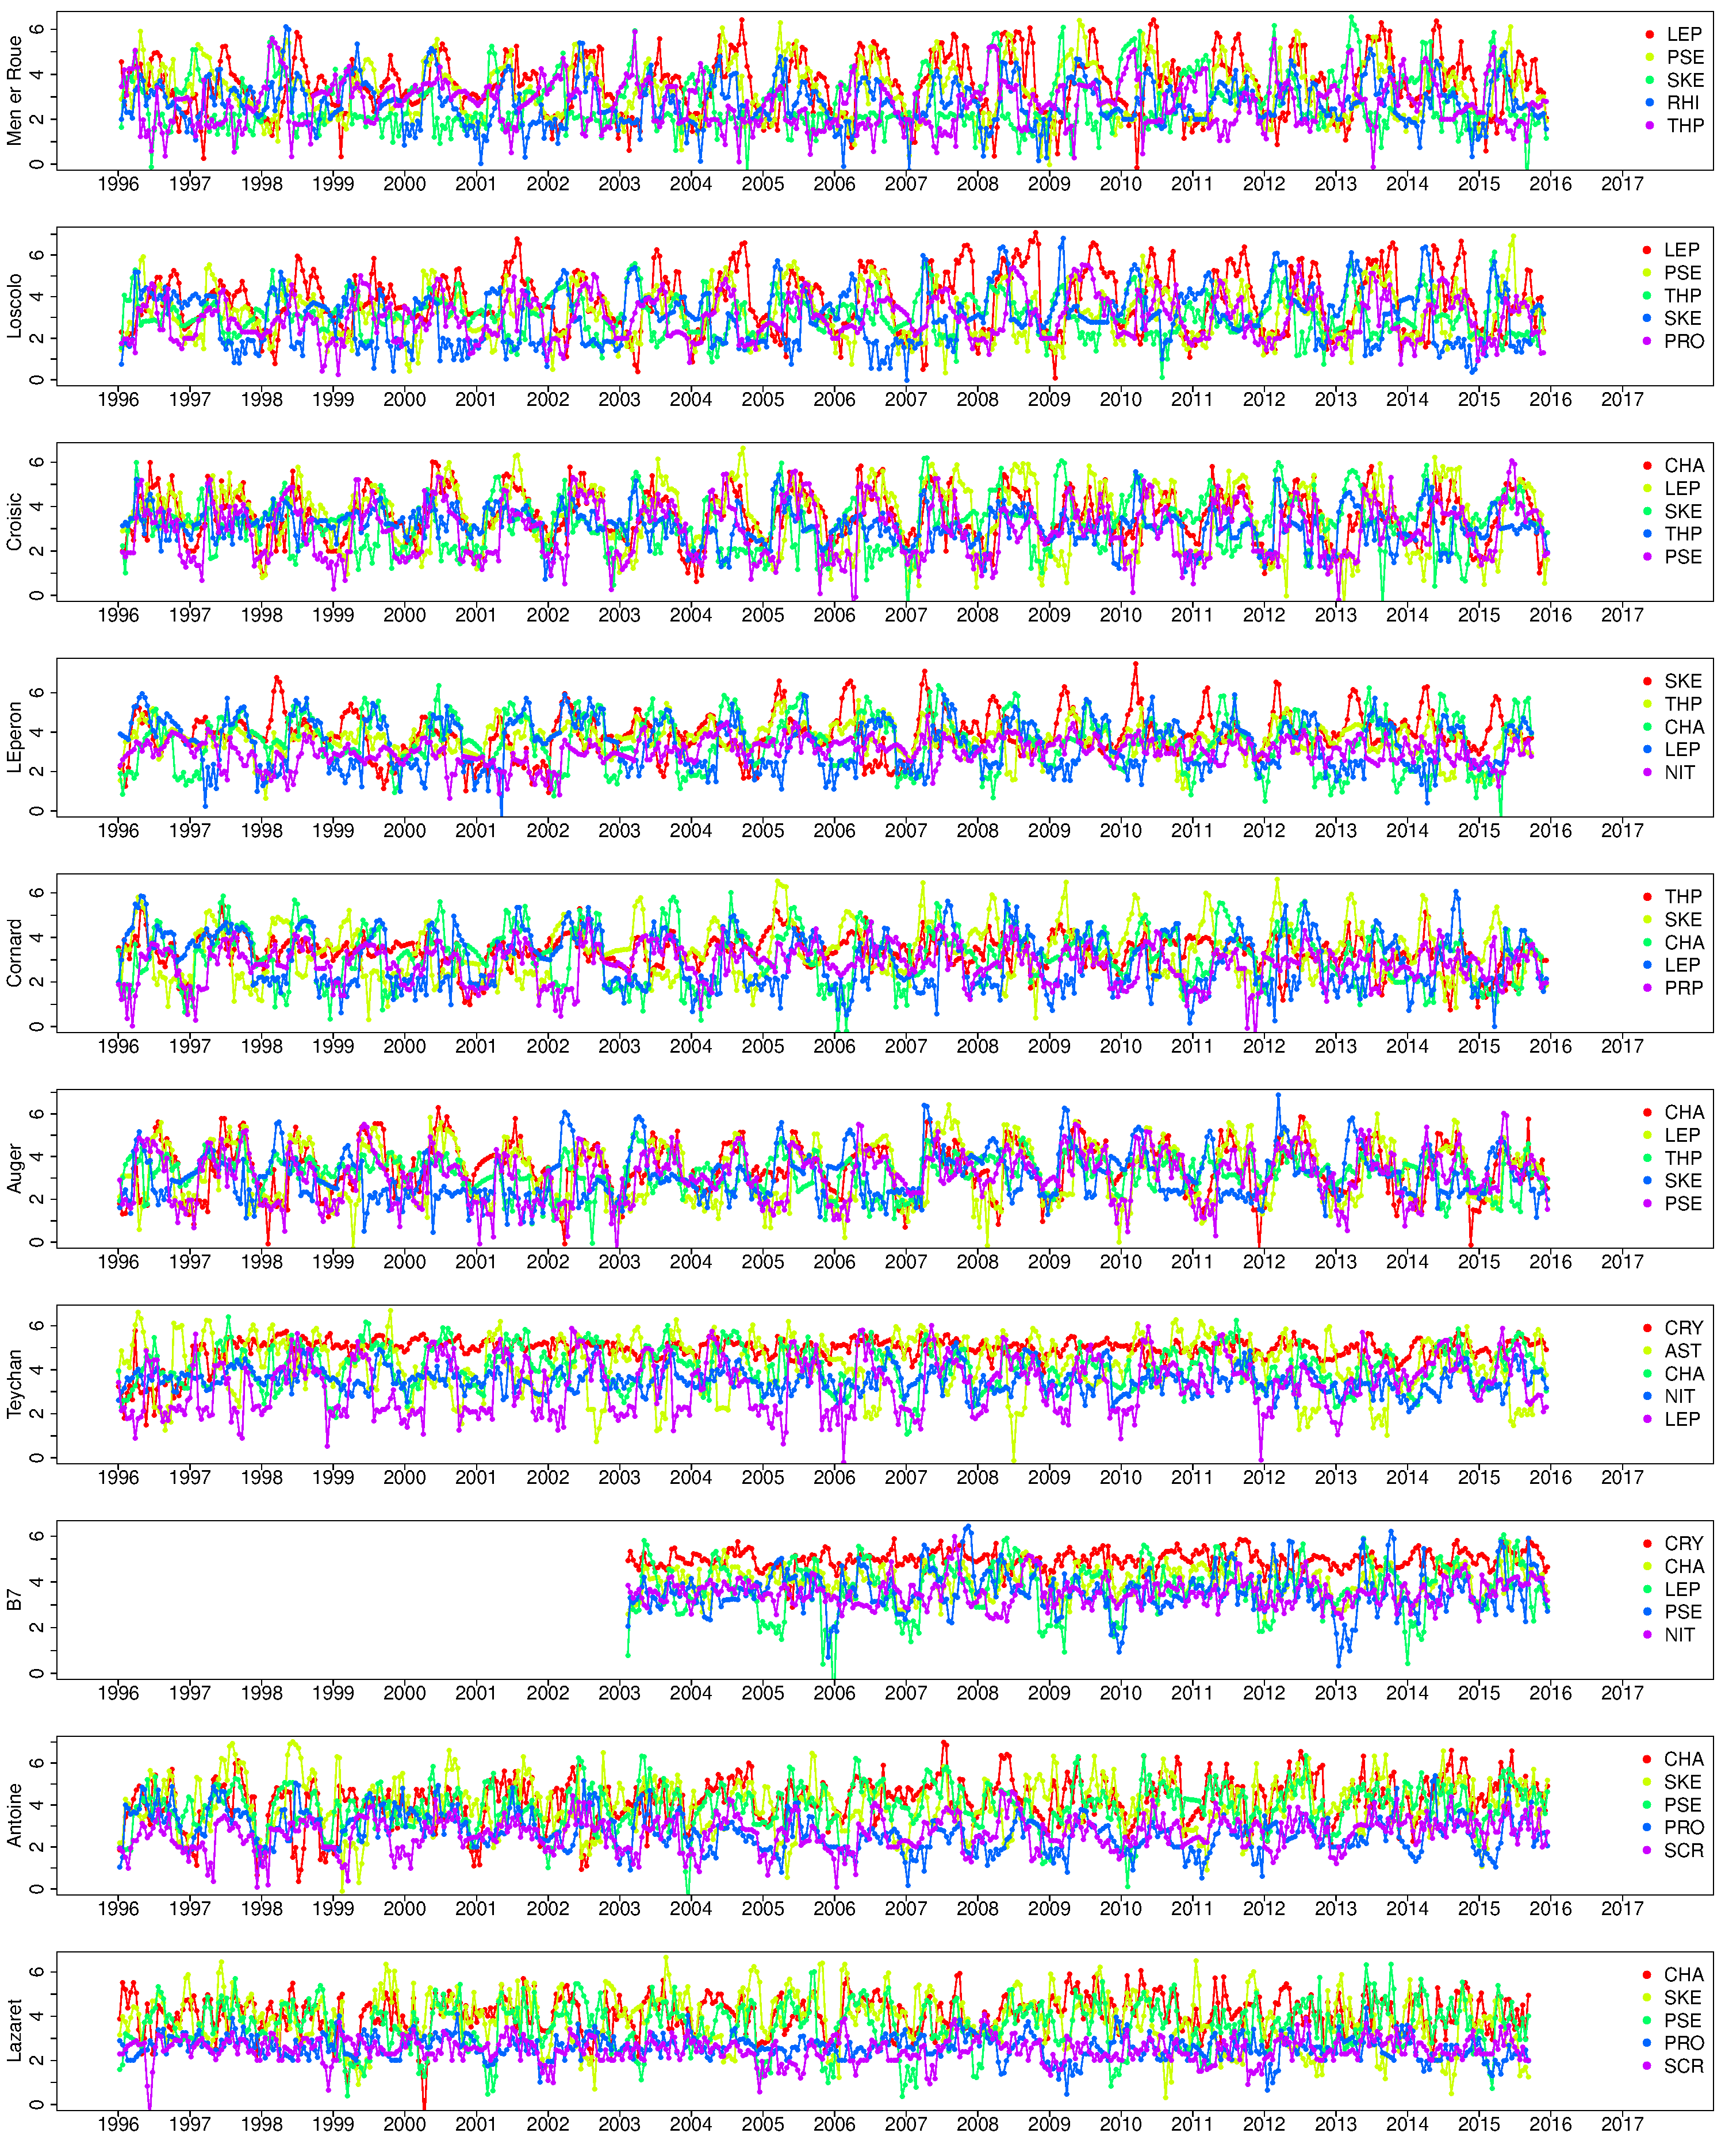
\includegraphics[width=0.99\textwidth]{time_series_plankton_site_by_site_most_abundant}
\par\end{centering}
\caption{\textbf{Time series of the 5 most abundant phytoplanktonic genera
in each site.\label{fig:Time-series}}}
\end{figure}


\subsection*{MAR(1) models}

We selected the most parsimonious interaction matrices using BIC.
Not only the best-ranking model, but also the overall ranking of interaction
scenarios were similar for most sites (Fig.~\ref{fig:Comparison-of-BIC}).
Based on these results, we considered the model selection to be quite
robust, and focused on the pennate-centric scenario to analyze interaction
matrices, as this scenario corresponded to the best fitted models
that still allowed interactions between groups.

\begin{figure}[H]
\begin{centering}
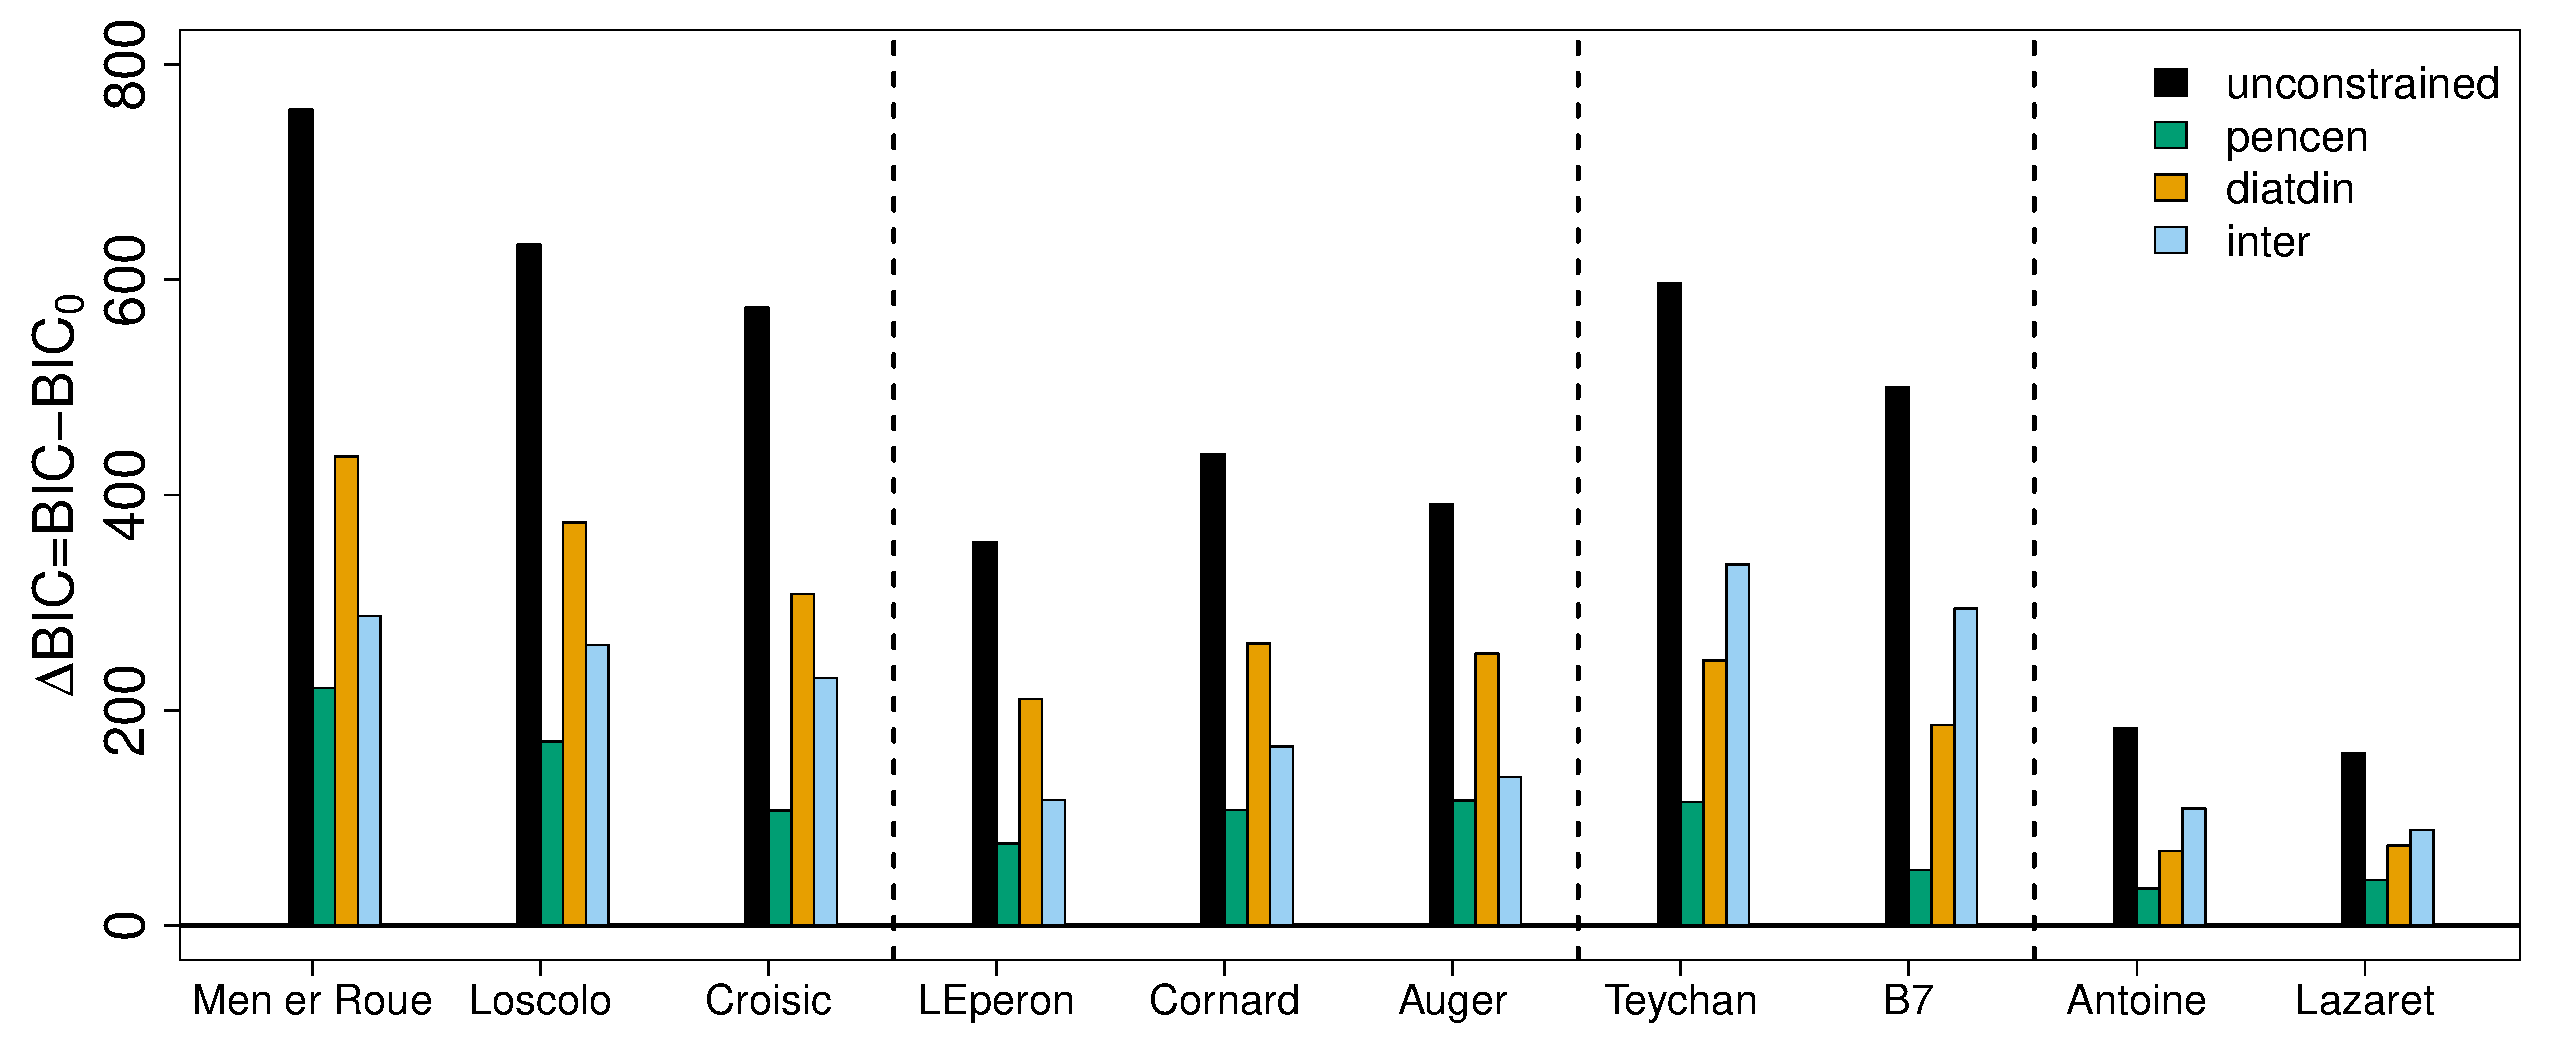
\includegraphics[width=0.99\textwidth]{comp_BIC_per_site}
\par\end{centering}
\caption{\textbf{Comparison of the BIC of different interaction scenarios},
compared to the null scenario (diagonal interaction matrix, allowing
only intragroup interactions), for 10 sites in 4 different regions,
separated by dashed lines (Brittany, Ol�ron, Arcachon and the Mediterranean
Sea). Different interaction matrices may allow interactions between
all taxa (unconstrained), only interactions within pennate diatoms,
centric diatoms, dinoflagellates, or other phytoplanktonic taxa (pencen),
only interactions within diatoms, dinoflagellates or other taxa (diatdin),
or only interactions between taxa belonging to these different groups
(inter). As data structures (length of the times series) are different between sites and regions, groups of bars should
not be compared.\label{fig:Comparison-of-BIC}}
\end{figure}

We inspected the Hessian matrices (i.e., Hessians of the negative
log-likelihood which is the observed Fisher Information Matrix) for
interaction parameters in order to check that results
presented in Fig. 3 of the main text could not be due to statistical
constraints. Correlation matrices (derived from the Hessian matrices)
showed that the mean absolute value of the correlation was 0.02 (hence
on average there were no correlations), few of those were noticeable
(75\% were below 0.1 in only 1 site, even lower in the 9 other sites)
and even the very few large ones were never above 0.5 in absolute
value.

In addition to the coefficients of the interaction matrix, MAR(1)
models allowed us to estimate the effect of environmental variables.
The regression coefficients reveal abiotic effects such as phenology
(temperature, related to insolation) or responses to hydrological
changes such as salinity variation (Fig.~\ref{fig:Abiotic_effects}).
Overall, temperature tended to have more effect on phytoplankton dynamics
than salinity, which {\color{blue}is} logical since it integrates seasonal variation
in received solar energy. The absolute effect of temperature was on
average 3.5 times higher than salinity effects and temperature coefficients
were significant at the 95\% threshold for 68\% of all estimates,
as opposed to 16\% for salinity effects. Temperature had a positive
effect in 80\% of the cases while salinity had a negative effect for
66\% of all estimates. The sign of significant temperature effects
on a given species remained the same between regions, except for SKE,
which was negatively affected by temperature in Brittany and Ol�ron
but positively affected by temperature in the Mediterranean Sea.

\begin{figure}[H]
\begin{centering}
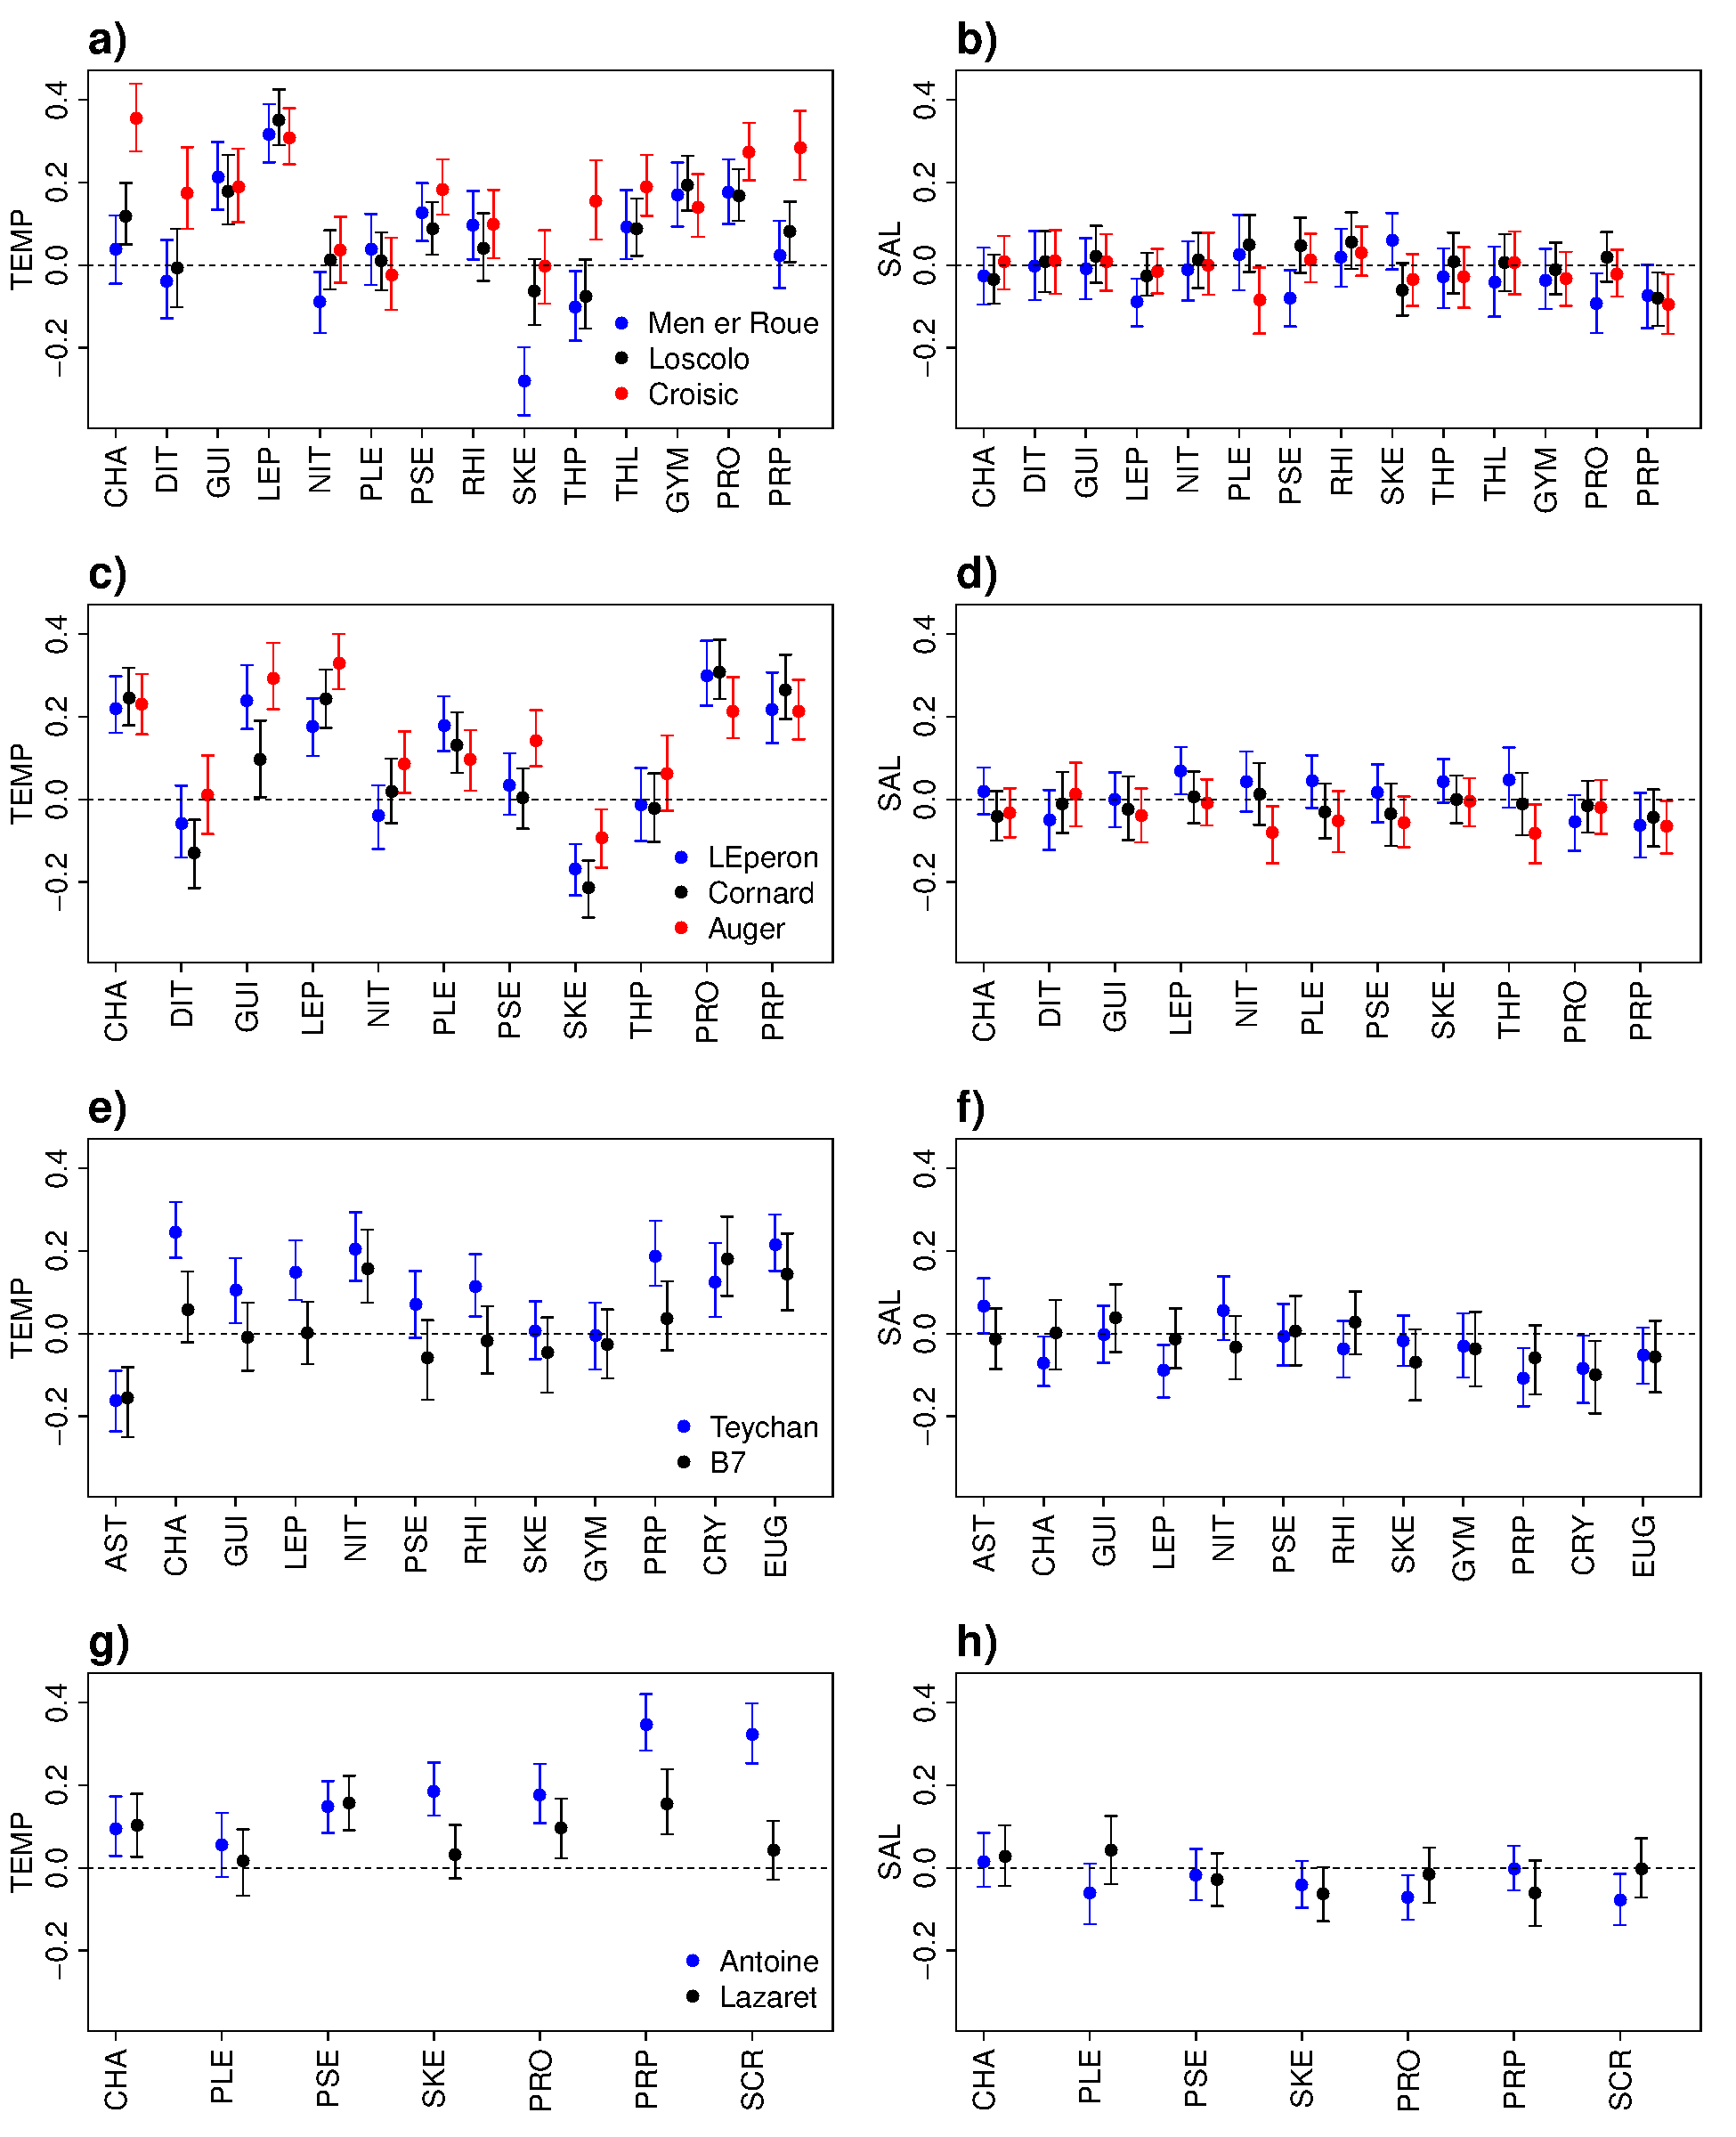
\includegraphics[width=0.99\textwidth]{abiotic_second_try}
\par\end{centering}
\caption{\textbf{Effect of environmental variables (temperature, TEMP or salinity,
SAL) on phytoplankton genera} in Brittany (a, b), Ol�ron (c, d), Arcachon
(e, f) and in the Mediterranean Sea (g, h). Each color corresponds
to a different site. Error bars correspond to the 95\% confidence
interval around the estimated coefficient. All variables were normalized
before estimation. \label{fig:Abiotic_effects}}
\end{figure}


\subsection*{Network analysis}

\subsubsection*{Interaction types}

\begin{figure}[H]
\begin{centering}
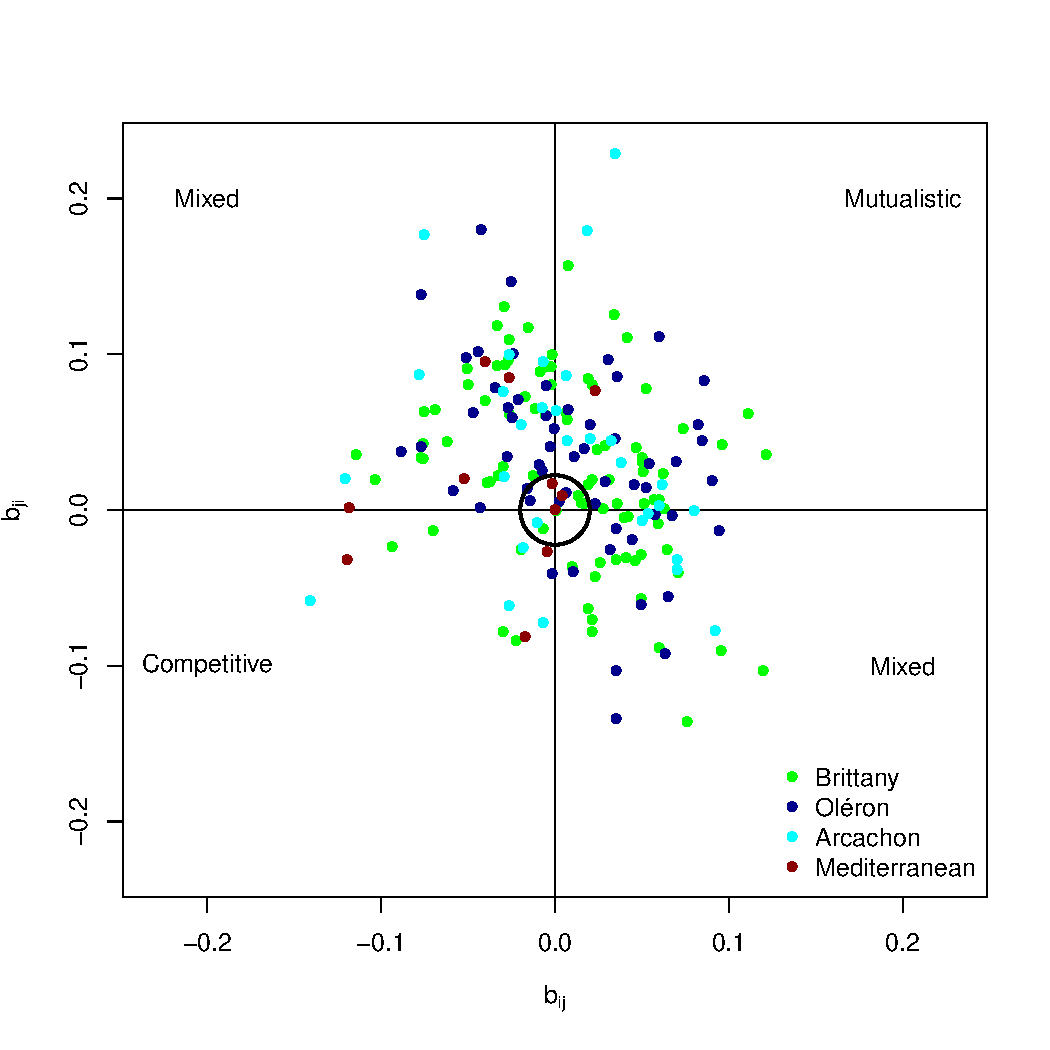
\includegraphics[width=0.95\textwidth]{pair_coefficients}
\par\end{centering}
\caption{\textbf{Pairs of coefficients for each study site}. The effect of
species $i$ on $j$ is given as a function of the effect of species
$j$ on species $i$. The black circle indicates the first quartile
of the interaction values, under which we can assume that the effect
is weak or null. Below this limit, (+/+), (+/-) or (-/+) interactions
can translate into commensalism or amensalism. Above, they can be
respectively mutualistic or mixed (+/-) links.\label{fig:Pairs-of-coefficients}}
\end{figure}


\subsubsection*{Metrics}

We characterised each interaction network with 3 quantitative descriptors:
the mean and variance of the intra- and intergenus coefficients (i.e.,
on and off the matrix diagonal) and the weighted
connectance of $\mathbf{B}\lyxmathsym{\textendash}\mathbf{I}$. The mean of absolute
values of intragenus coefficients was approximately 8 times higher
than the mean of the absolute values of the effect of intergenus interactions. The intragenus
interactions' variance was about 4 times higher than the variance of intergenus interactions (Fig.~\ref{fig:MeanVar}).

\begin{figure}[H]
\begin{centering}
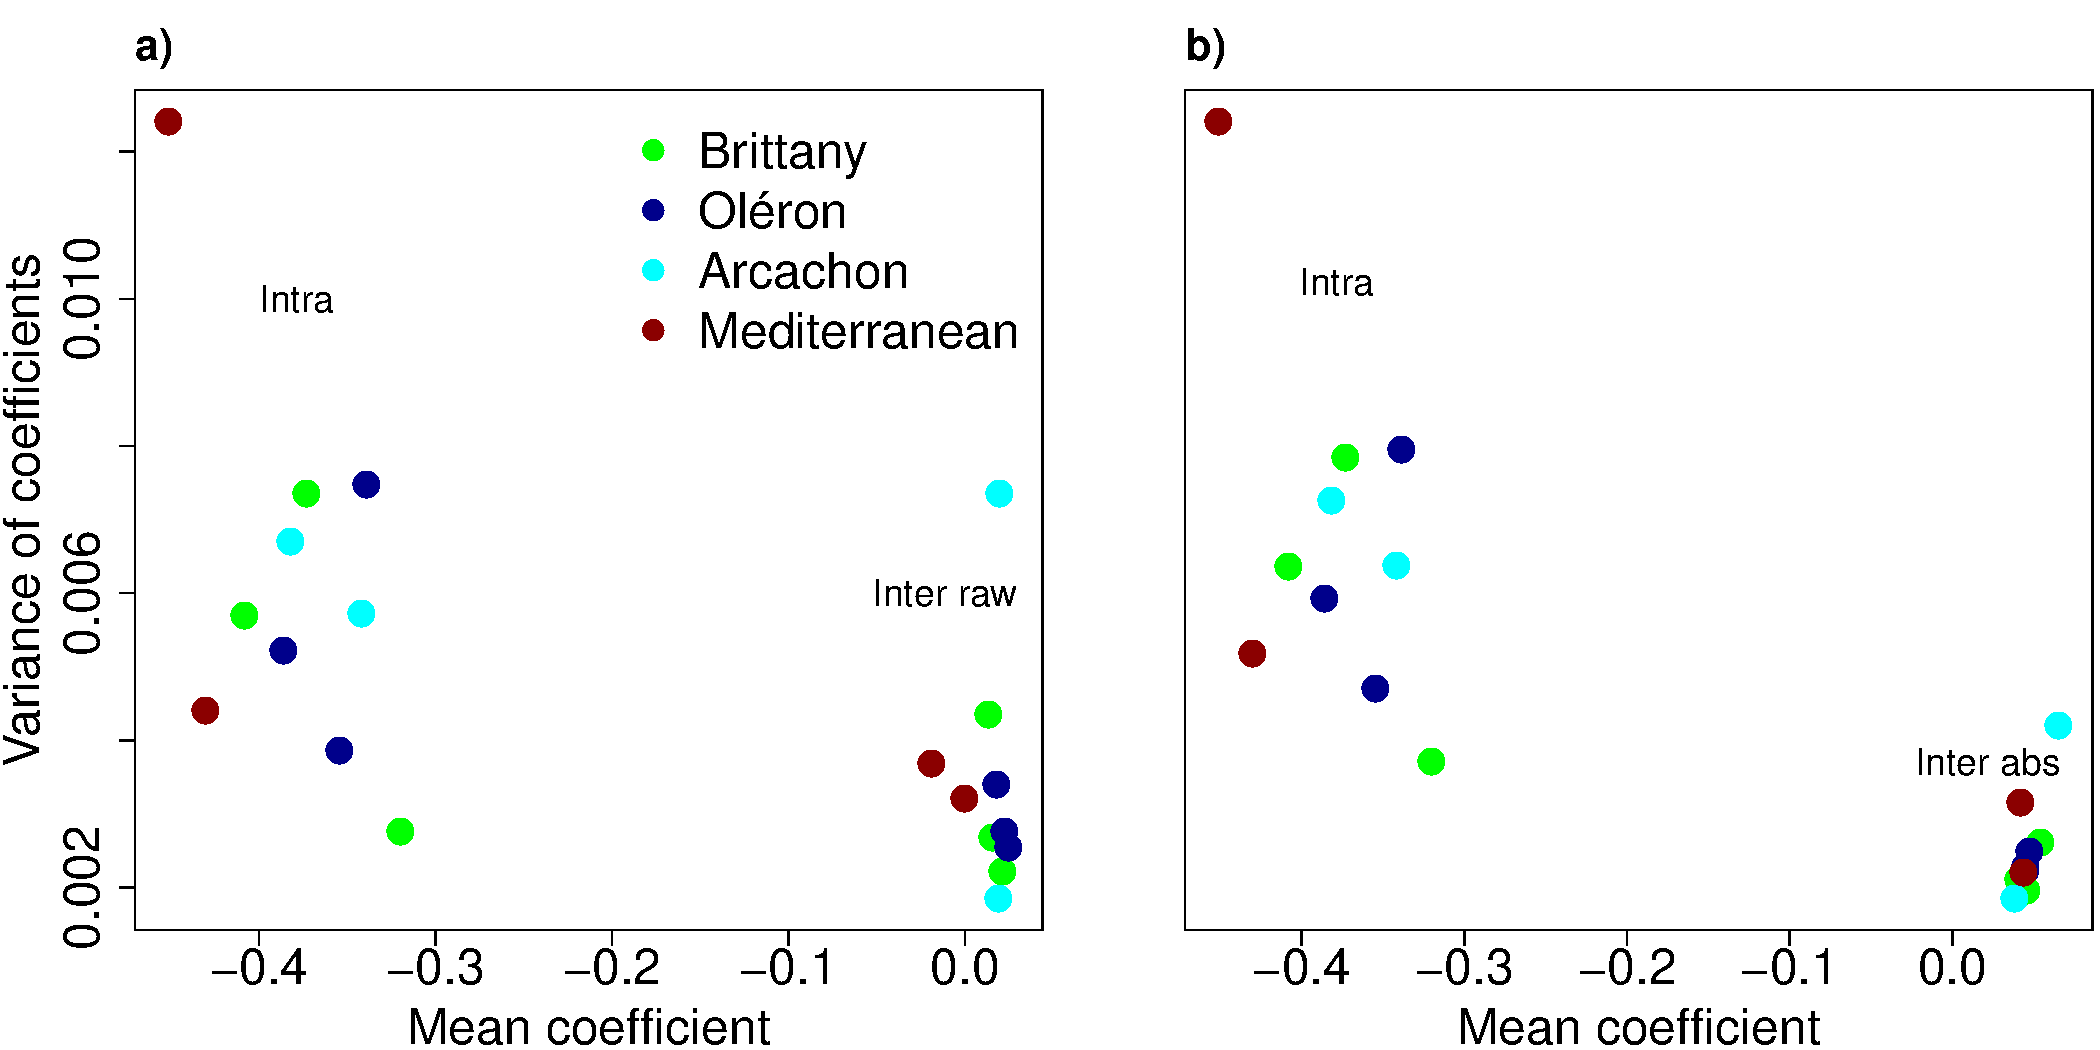
\includegraphics[width=0.99\textwidth]{moy_vs_var_for_all_interactions_pencen_SI}
\par\end{centering}
\caption{\textbf{Relation between mean and variance of the intra- and intergenus
interaction coefficients}. The variance of the coefficients in the
interaction matrix $(\mathbf{B}\text{\textendash}\mathbf{I})$ increases
with the mean, for 10 sites in 4 regions, with a model allowing interactions
only within clads (within centric or pennate diatoms, dinoflagellates,
or other taxa). The mean-variance relation was either computed with
raw values of intergroup interactions (a) or absolute values of the
intergroup coefficients (b). We did not take the absolute value of intragroup coefficients since they were all negative.
\label{fig:MeanVar}}
\end{figure}

The intragenus interaction strength could be related to the mean abundance
of each genus as the most self-regulated genera were also the least
abundant (Fig.~\ref{fig:IntraVAbundance}).

\begin{figure}[H]
\begin{centering}
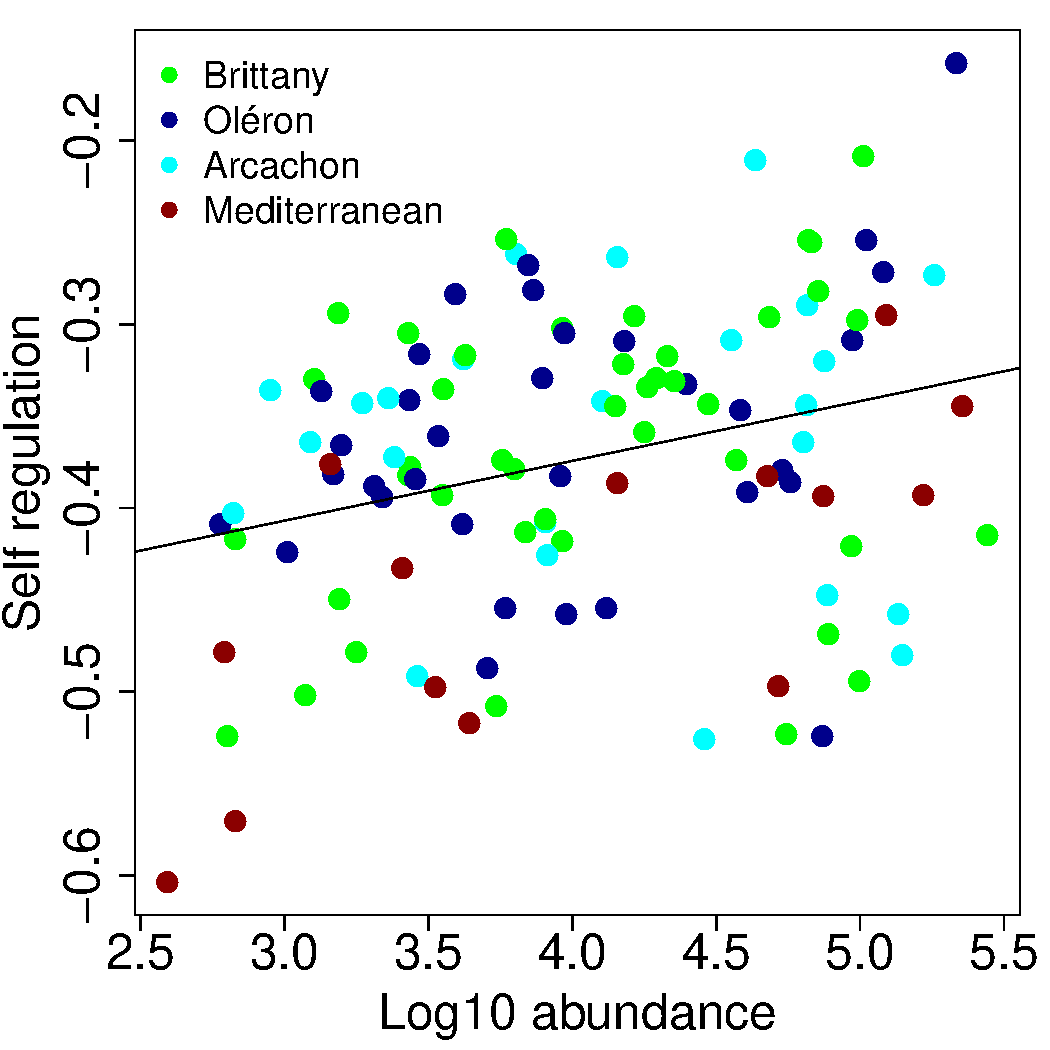
\includegraphics[width=0.45\textwidth]{abundance_vs_regulation}
\par\end{centering}
\caption{\textbf{Relation between abundance and self-regulation} (intragenus
interaction coefficients). Mean abundance is computed for each genus
in each site in 4 regions and intragenus interaction strengths are
the diagonal coefficients of the interaction matrix $(\mathbf{B}\text{\textendash}\mathbf{I})$.
\label{fig:IntraVAbundance}}
\end{figure}

Weighted connectance is described in \citet{bersier_quantitative_2002}. It is based on the average of vulnerability and generality in the network. More precisely, diversity measures of the interactions from ($H_{P,k}$)
and to ($H_{N,k}$) the phytoplanktonic group $k$ can be computed
as:

\begin{equation}
H_{N,k}=-\sum_{i=1}^{S}\frac{b_{ik}}{b_{\centerdot k}}\log_{2}\left(\frac{b_{ik}}{b_{\centerdot k}}\right)\label{eq:DiversityIn}
\end{equation}

\begin{equation}
H_{P,k}=-\sum_{i=1}^{S}\frac{b_{ki}}{b_{k\centerdot}}\log_{2}\left(\frac{b_{ki}}{b_{k\centerdot}}\right)\label{eq:DiversityOut}
\end{equation}

where $b_{ik}$ is a coefficient of the interaction matrix $(\mathbf{B}\text{\textendash}\mathbf{I})$,
$b_{k\centerdot}=\sum_{i=1}^{S}b_{ki}$ is the sum of all coefficients
over row $k$ and $S$ is the number of species in the network. These
indices are then averaged for the whole network as the linkage density
$LD$ (eq. \ref{eq:LD}).

\begin{equation}
LD=\frac{1}{2}\left(\sum_{k=1}^{S}\frac{b_{\centerdot k}}{b_{\centerdot\centerdot}}2^{H_{N,k}}+\sum_{k=1}^{S}\frac{b_{k\centerdot}}{b_{\centerdot\centerdot}}2^{H_{P,k}}\right)\label{eq:LD}
\end{equation}

where $b_{\centerdot\centerdot}=\sum_{j=1}^{S}\sum_{i=1}^{S}b_{ji}$
is the sum of all coefficients of the interaction matrix $(\mathbf{B}\text{\textendash}\mathbf{I})$.

Weighted connectance $C$ is then defined as:

\begin{equation}
C=\frac{LD}{S}\label{eq:Weighted_connectance}
\end{equation}

Contrary to linkage density, weighted connectance accounts for the
dimension of the interaction matrix and can be used to compare network
in different regions, with different dimensions.

In addition to this network-level metric, we also considered metrics
for each phytoplanktonic group. We measured both its vulnerability
(mean strength of the interactions that are applied to a group, eq.~\ref{eq:vulnerability})
and its impact (mean strength of the interactions the group applies
to other groups, eq.~\ref{eq:impact}) in each network.

\begin{equation}
v_{k}=\mathnormal{\frac{1}{\boldsymbol{1}_{\mathnormal{b_{ki}\neq0}}}}\sum_{i=1}^{S}b_{ki}\label{eq:vulnerability}
\end{equation}

\begin{equation}
e_{k}=\frac{1}{\boldsymbol{1}_{\mathnormal{b_{ik}\neq0}}}\sum_{i=1}^{S}b_{ik}\label{eq:impact}
\end{equation}

where $\boldsymbol{1}_{\mathnormal{b_{ki}\neq0}}$ is the number of
interactions which are different from 0 in row $k$.

\subsection*{Comparison with a full interaction matrix}

We checked that, by choosing the model with the lowest BIC, we did not miss interactions which would have changed our conclusions. To do so, we examined the full (unconstrained) model results for all study sites. We present those results below (Fig. \ref{fig:unconstrained} and Table \ref{table:unconstrained}). 

\begin{figure}[H]
    \centering
    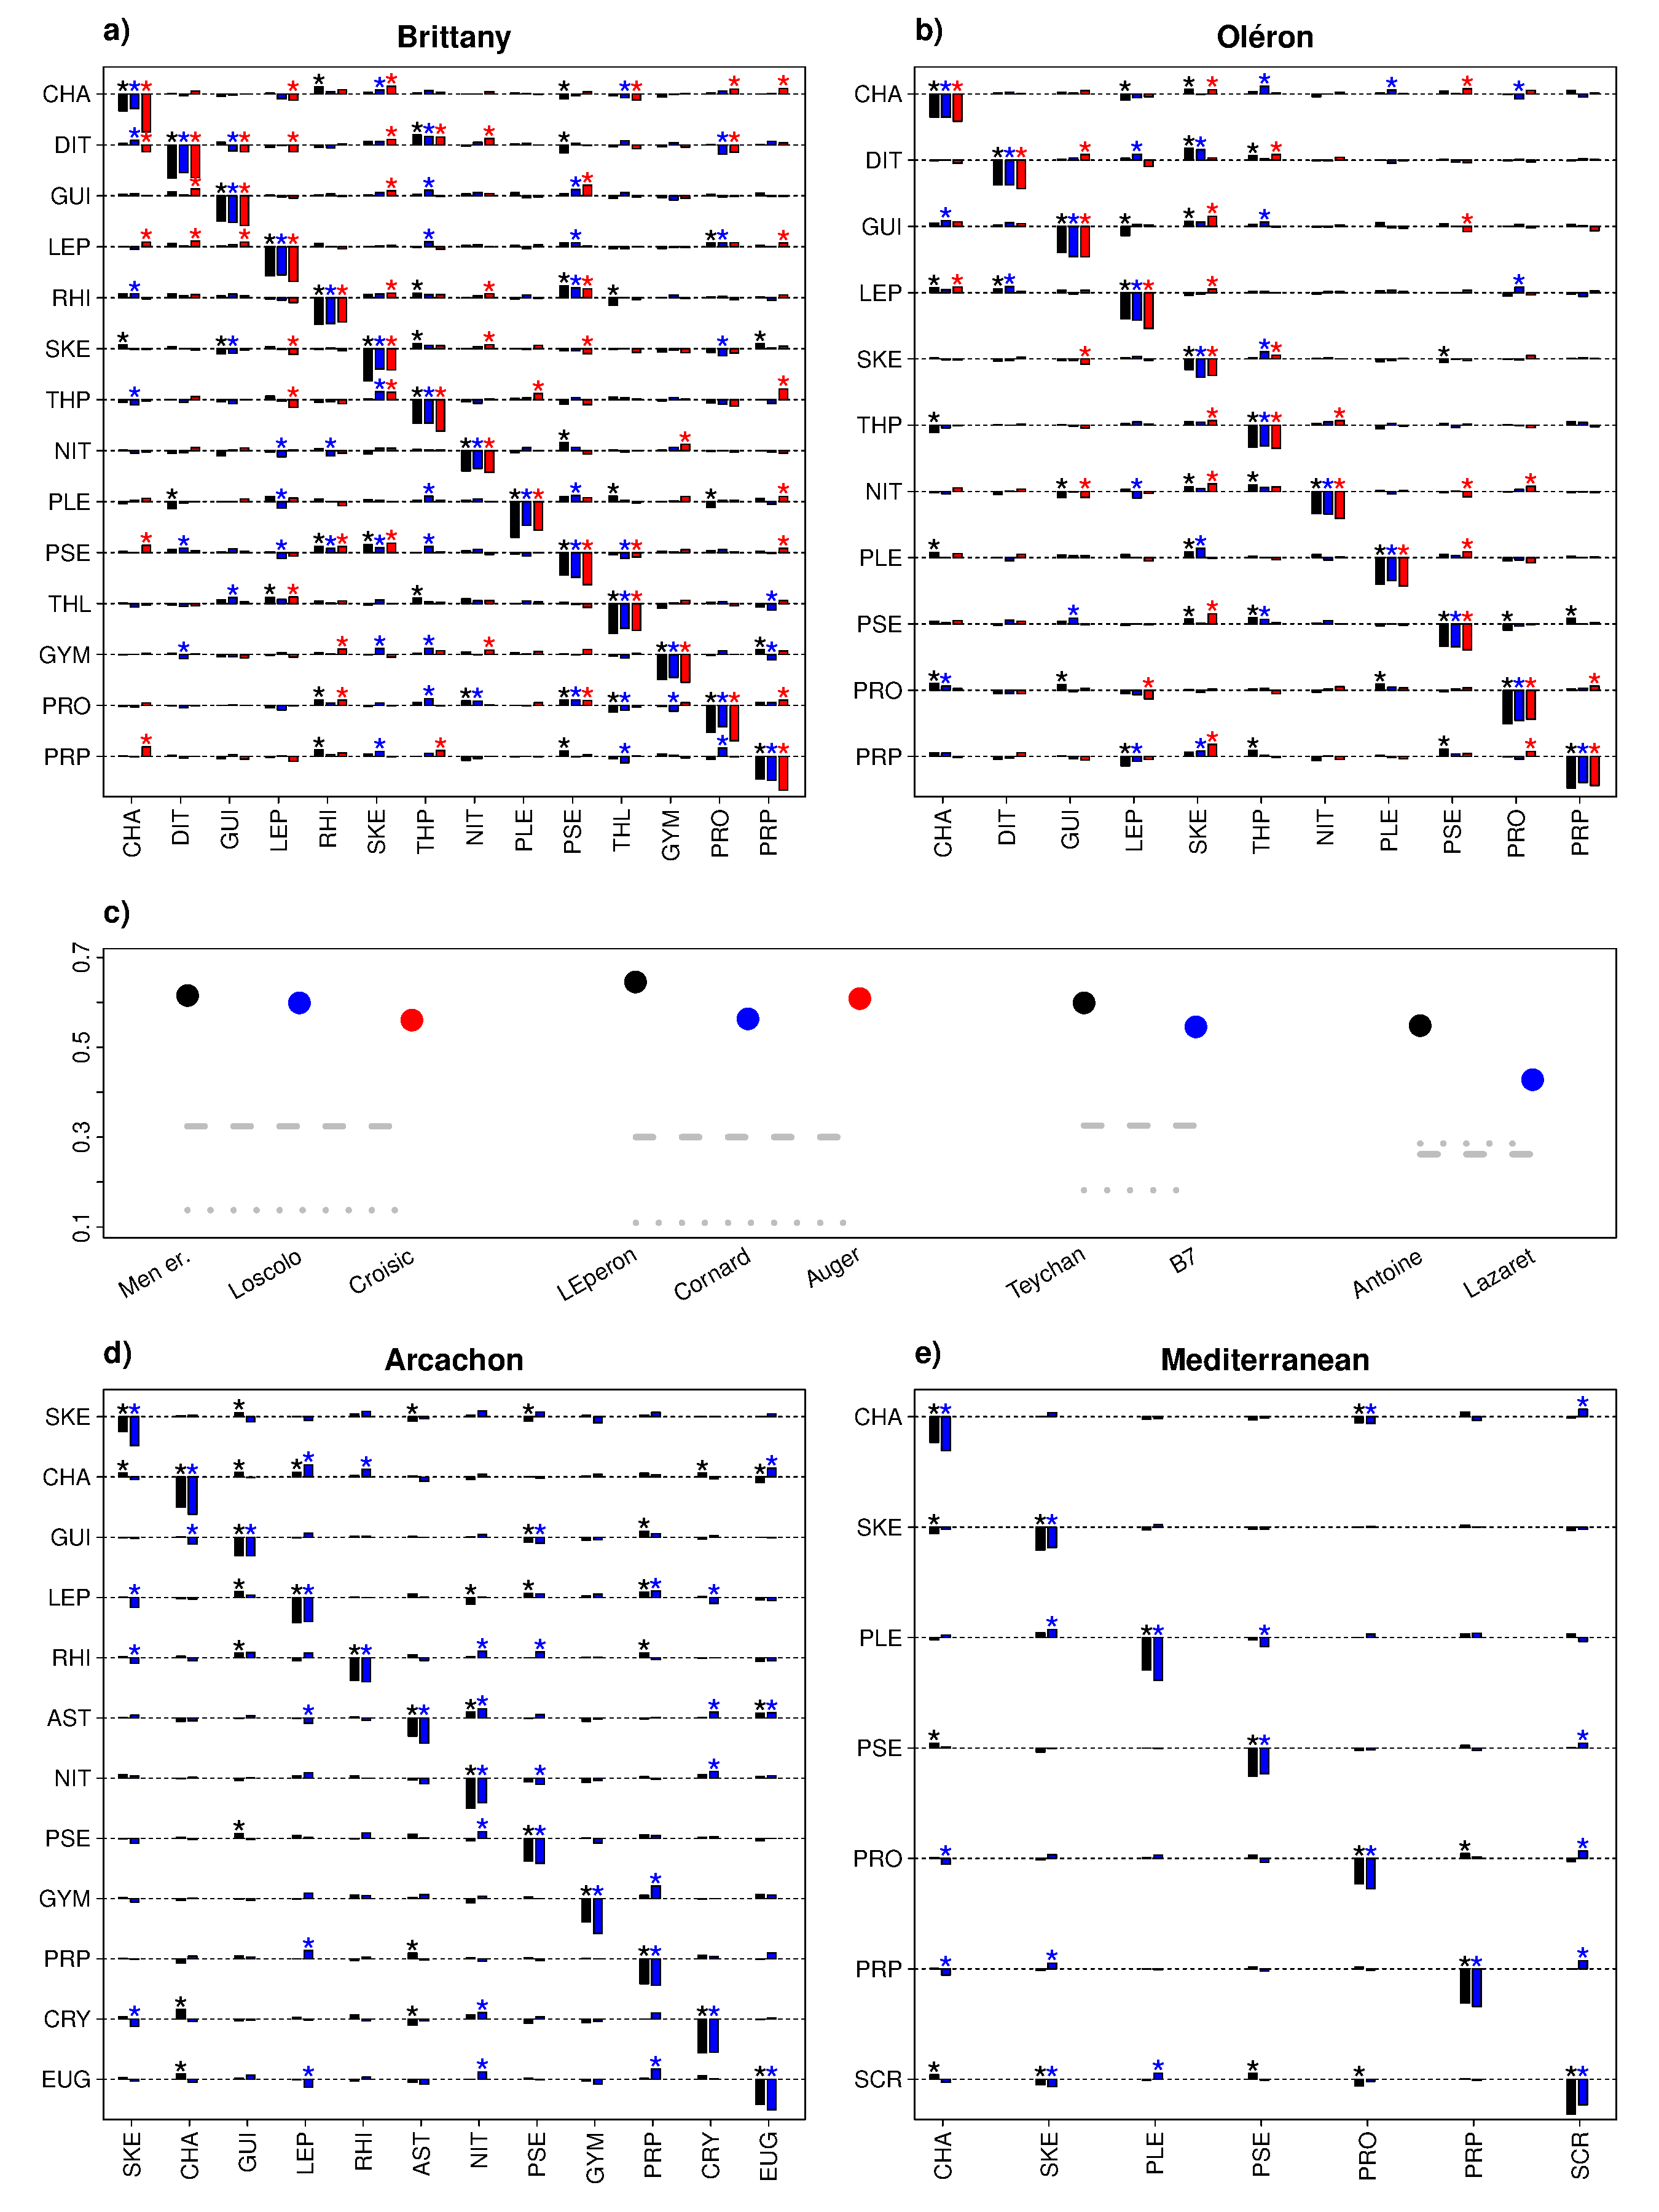
\includegraphics[width=0.90\linewidth]{biotic_interaction_matrices_unconstrained.pdf}
    \caption{Interaction matrices estimated in 10 sites along the French coastline. Four regions are distinguished: Brittany (a), Ol�ron (b), Arcachon (d) and the Mediterranean Sea (e). There is no constraint on the structure (modularity) of the interaction matrices. The fraction of positive interactions in each matrix is given by points in c) while the dashed (resp., dotted) line represents the ratio of interactions remaining positive (resp., negative) for all sites of a given region.}
    \label{fig:unconstrained}
\end{figure}

\begin{table}[ht]
\centering
 \begin{adjustbox}{max width=\textwidth}
\begin{tabular}{ccccccccc}
  \hline
 & signif outside & positive & ratio intra/inter & ratio in/out block & transfo sign \\ 
  \hline
Men er Roue & 0.09 & 0.57 & 11.06 & 3.03 & 0.04 \\ 
  Loscolo & 0.14 & 0.56 & 8.42 & 2.65 & 0.07 \\ 
  Croisic & 0.13 & 0.52 & 10.15 & 2.89 & 0.09 \\ 
  LEperon & 0.13 & 0.59 & 8.78 & 2.75 & 0.04 \\ 
  Cornard & 0.08 & 0.51 & 10.32 & 3.64 & 0.06 \\ 
  Auger & 0.07 & 0.55 & 9.66 & 3.10 & 0.06 \\ 
  Antoine & 0.10 & 0.47 & 11.18 & 5.21 & 0.00 \\ 
  Lazaret & 0.18 & 0.37 & 8.67 & 4.30 & 0.00 \\ 
  Teychan & 0.11 & 0.55 & 10.46 & 3.68 & 0.14 \\ 
  B7 & 0.11 & 0.50 & 8.29 & 3.59 & 0.14 \\ 
   \hline
\end{tabular}
\end{adjustbox}
\caption{Descriptors of coefficients in unconstrained interaction matrices and comparison to best-fitting pennate-centric structures: ratio of coefficients significantly different from 0 outside of the pennate-centric blocks vs total number of coefficients in the unconstrained matrix, proportion of positive interactions in the unconstrained matrix, ratio of mean intragroup interaction strength and mean intergroup interaction strength in the unconstrained matrix, ratio of mean interaction strength inside the pennate-centric modules vs outside the pennate-centric modules in the unconstrained matrix and proportion of interactions changing sign between the two structures.}
\label{table:unconstrained}
\end{table}

Thus, even if we chose to select the full interaction model, there would be no difference in our main conclusions: intragenus interactions are much stronger than intergenus interactions and positive interactions are still the rule. There is at most 18\% of interactions significantly different from zero outside of the pennate and centric blocks and those interactions are on average 3.5 times lower than the interactions inside the pennate and centric blocks (Table \ref{table:unconstrained}).

\subsection*{MAR references and analysis}

%%%%%PUT THAT HERE : 

We present here the MAR references we used to compare the effects
of intra- and intergroup interactions (Table~\ref{tab:Studies},
Fig.~\ref{fig:Ratio-of-intra-to-intergroup}). We add
information on the biome and taxa used in the study as they tend to
be linked to the estimated parameters (Fig.~\ref{fig:ratio_meta}). We should mention two potential biases associated with this
comparison across the published literature. First, low-dimensional
matrices tended to be more complete (less sparse) than high-dimensional
matrices, as these small interaction matrices were used to study known
interaction phenomena (observed predation between organisms, for instance). In fact, we add pairs of predator and prey mainly to give a scale to the plot.
Conversely, the number of parameters to estimate increases as the
square of the number of interacting taxa, leading most authors to
reduce this set before the estimation process for large interaction
matrices. There is therefore a positive correlation between sparsity
and dimensionality (Fig.~\ref{fig:ratio_meta}). A second caveat is that while we informed
our model selection by phylogeny, several authors have
instead reduced the number of estimated parameters by an automated
procedure, usually based on the comparison of hundreds of randomly chosen
interaction matrices by AIC \citep{ives_community_1999}. The latter
choice is likely to bias high non-zero interactions in the literature.
This is why we decided to present in the main text intra/inter ratios
including interspecific (or intergroup) coefficients set to zero (see Fig. 4 in the main text),
which should be less sensitive to the model selection method and therefore
make comparisons across studies possible. In Fig.~\ref{fig:Ratio-of-intra-to-intergroup}, mean interaction strengths were computed as the mean absolute value
of only the set of coefficients which were deemed significant at the 95\% threshold
in the $(\mathbf{B}\text{\textendash}\mathbf{I})$ matrix.

\begin{sidewaystable}[H]
\begin{centering}
{\footnotesize{}}%
\begin{tabular}{ccccccc}
\hline 
\textbf{\footnotesize{}Code} & \textbf{\footnotesize{}Ref} & \textbf{\footnotesize{}Dimension} & \textbf{\footnotesize{}Type of organisms} & \textbf{\footnotesize{}Taxonomic level} & \textbf{\footnotesize{}System} & \textbf{\footnotesize{}T}\tabularnewline
\hline 
{\footnotesize{}1a} & {\footnotesize{}\citet{ives_community_1999}, CLS} & {\footnotesize{}9} & {\footnotesize{}Zooplankton} & {\footnotesize{}Species and functional groups} & {\footnotesize{}Lake} & {\footnotesize{}100}\tabularnewline
{\footnotesize{}1b} & {\footnotesize{}\citet{ives_community_1999}, TLS} & {\footnotesize{}9} & {\footnotesize{}Zooplankton} & {\footnotesize{}Species and functional groups} & {\footnotesize{}Lake} & {\footnotesize{}100}\tabularnewline
{\footnotesize{}2a} & {\footnotesize{}\citet{klug_compensatory_2000}} & {\footnotesize{}2} & {\footnotesize{}Phytoplankton} & {\footnotesize{}Phylum} & {\footnotesize{}Lake} & {\footnotesize{}100}\tabularnewline
{\footnotesize{}2b} & {\footnotesize{}\citet{klug_compensatory_2000}} & {\footnotesize{}3} & {\footnotesize{}Zooplankton} & {\footnotesize{}Species} & {\footnotesize{}Lake} & {\footnotesize{}50}\tabularnewline
{\footnotesize{}3a} & {\footnotesize{}\citet{klug_interactions_2001}} & {\footnotesize{}4} & {\footnotesize{}Functional groups of plankton} & {\footnotesize{}NA} & {\footnotesize{}Lake} & {\footnotesize{}300}\tabularnewline
{\footnotesize{}3b} & {\footnotesize{}\citet{klug_interactions_2001}} & {\footnotesize{}5} & {\footnotesize{}Taxonomic groups of plankton} & {\footnotesize{}Phylum/division} & {\footnotesize{}Lake} & {\footnotesize{}300}\tabularnewline
{\footnotesize{}4a} & {\footnotesize{}\citet{ives_estimating_2003}} & {\footnotesize{}4} & {\footnotesize{}Plankton} & {\footnotesize{}Zooplankton v. phytoplankton, size classes} & {\footnotesize{}Lake} & {\footnotesize{}100}\tabularnewline
{\footnotesize{}4b} & {\footnotesize{}\citet{ives_estimating_2003}} & {\footnotesize{}4} & {\footnotesize{}Plankton} & {\footnotesize{}Zooplankton v. phytoplankton, size classes} & {\footnotesize{}Lake with high planktivory} & {\footnotesize{}100}\tabularnewline
{\footnotesize{}4c} & {\footnotesize{}\citet{ives_estimating_2003}} & {\footnotesize{}4} & {\footnotesize{}Plankton} & {\footnotesize{}Zooplankton v. phytoplankton, size classes} & {\footnotesize{}Lake with low planktivory} & {\footnotesize{}100}\tabularnewline
{\footnotesize{}5a} & {\footnotesize{}\citet{hampton_empirical_2006}} & {\footnotesize{}14} & {\footnotesize{}Plankton} & {\footnotesize{}Phylum (phytoplankton), genus (zooplankton)} & {\footnotesize{}Lake} & {\footnotesize{}300}\tabularnewline
{\footnotesize{}5b} & {\footnotesize{}\citet{hampton_empirical_2006}} & {\footnotesize{}14} & {\footnotesize{}Plankton, growing season} & {\footnotesize{}Phylum (phytoplankton), genus (zooplankton)} & {\footnotesize{}Lake} & {\footnotesize{}200}\tabularnewline
{\footnotesize{}6a} & {\footnotesize{}\citet{hampton_coalescence_2006}} & {\footnotesize{}13} & {\footnotesize{}Plankton} & {\footnotesize{}Phyum (phytoplankton), genus (zooplankton)} & {\footnotesize{}Lake} & {\footnotesize{}400}\tabularnewline
{\footnotesize{}6b} & {\footnotesize{}\citet{hampton_coalescence_2006}} & {\footnotesize{}7} & {\footnotesize{}Simpler web, plankton} & {\footnotesize{}Phylum (phytoplankton), genus (zooplankton)} & {\footnotesize{}Lake} & {\footnotesize{}400}\tabularnewline
{\footnotesize{}7a} & {\footnotesize{}\citet{huber_role_2006}} & {\footnotesize{}10} & {\footnotesize{}Ciliates} & {\footnotesize{}Genus and species} & {\footnotesize{}Lake} & {\footnotesize{}300}\tabularnewline
{\footnotesize{}7b} & {\footnotesize{}\citet{huber_role_2006}} & {\footnotesize{}10} & {\footnotesize{}Phytoplankton} & {\footnotesize{}Genus and species} & {\footnotesize{}Lake} & {\footnotesize{}300}\tabularnewline
{\footnotesize{}8a} & {\footnotesize{}\citet{yamamura_how_2006}} & {\footnotesize{}3} & {\footnotesize{}Insects} & {\footnotesize{}Species} & {\footnotesize{}Terrestrial} & {\footnotesize{}50}\tabularnewline
{\footnotesize{}9a} & {\footnotesize{}\citet{vik_interlinking_2008}} & {\footnotesize{}2} & {\footnotesize{}Lynx/Hare} & {\footnotesize{}Species} & {\footnotesize{}Terrestrial} & {\footnotesize{}100}\tabularnewline
{\footnotesize{}10a} & {\footnotesize{}\citet{lindegren_preventing_2009}} & {\footnotesize{}3} & {\footnotesize{}Fish} & {\footnotesize{}Species} & {\footnotesize{}Baltic Sea} & {\footnotesize{}30}\tabularnewline
{\footnotesize{}11a} & {\footnotesize{}\citet{griffiths_phytoplankton_2015}} & {\footnotesize{}7} & {\footnotesize{}Phytoplankton} & {\footnotesize{}Phylum} & {\footnotesize{}Coastal site} & {\footnotesize{}1000}\tabularnewline
{\footnotesize{}11b} & {\footnotesize{}\citet{griffiths_phytoplankton_2015}} & {\footnotesize{}7} & {\footnotesize{}Phytoplankton} & {\footnotesize{}Phylum} & {\footnotesize{}Offshore site} & {\footnotesize{}700}\tabularnewline
{\footnotesize{}12a} & {\footnotesize{}\citet{barraquand_coastal_2018}} & {\footnotesize{}12} & {\footnotesize{}Phytoplankton} & {\footnotesize{}Genus} & {\footnotesize{}Outside a bay} & {\footnotesize{}300}\tabularnewline
{\footnotesize{}12b} & {\footnotesize{}\citet{barraquand_coastal_2018}} & {\footnotesize{}12} & {\footnotesize{}Phytoplankton} & {\footnotesize{}Genus} & {\footnotesize{}Inside a bay} & {\footnotesize{}500}\tabularnewline
\end{tabular}{\footnotesize\par}
\par\end{centering}
\caption{Studies used when comparing |intra|/|inter| ratios in Fig. 4 in main
text.
T is the approximate number of sampling dates in each time series.
\label{tab:Studies}}
\end{sidewaystable}

\begin{figure}[H]
\begin{centering}
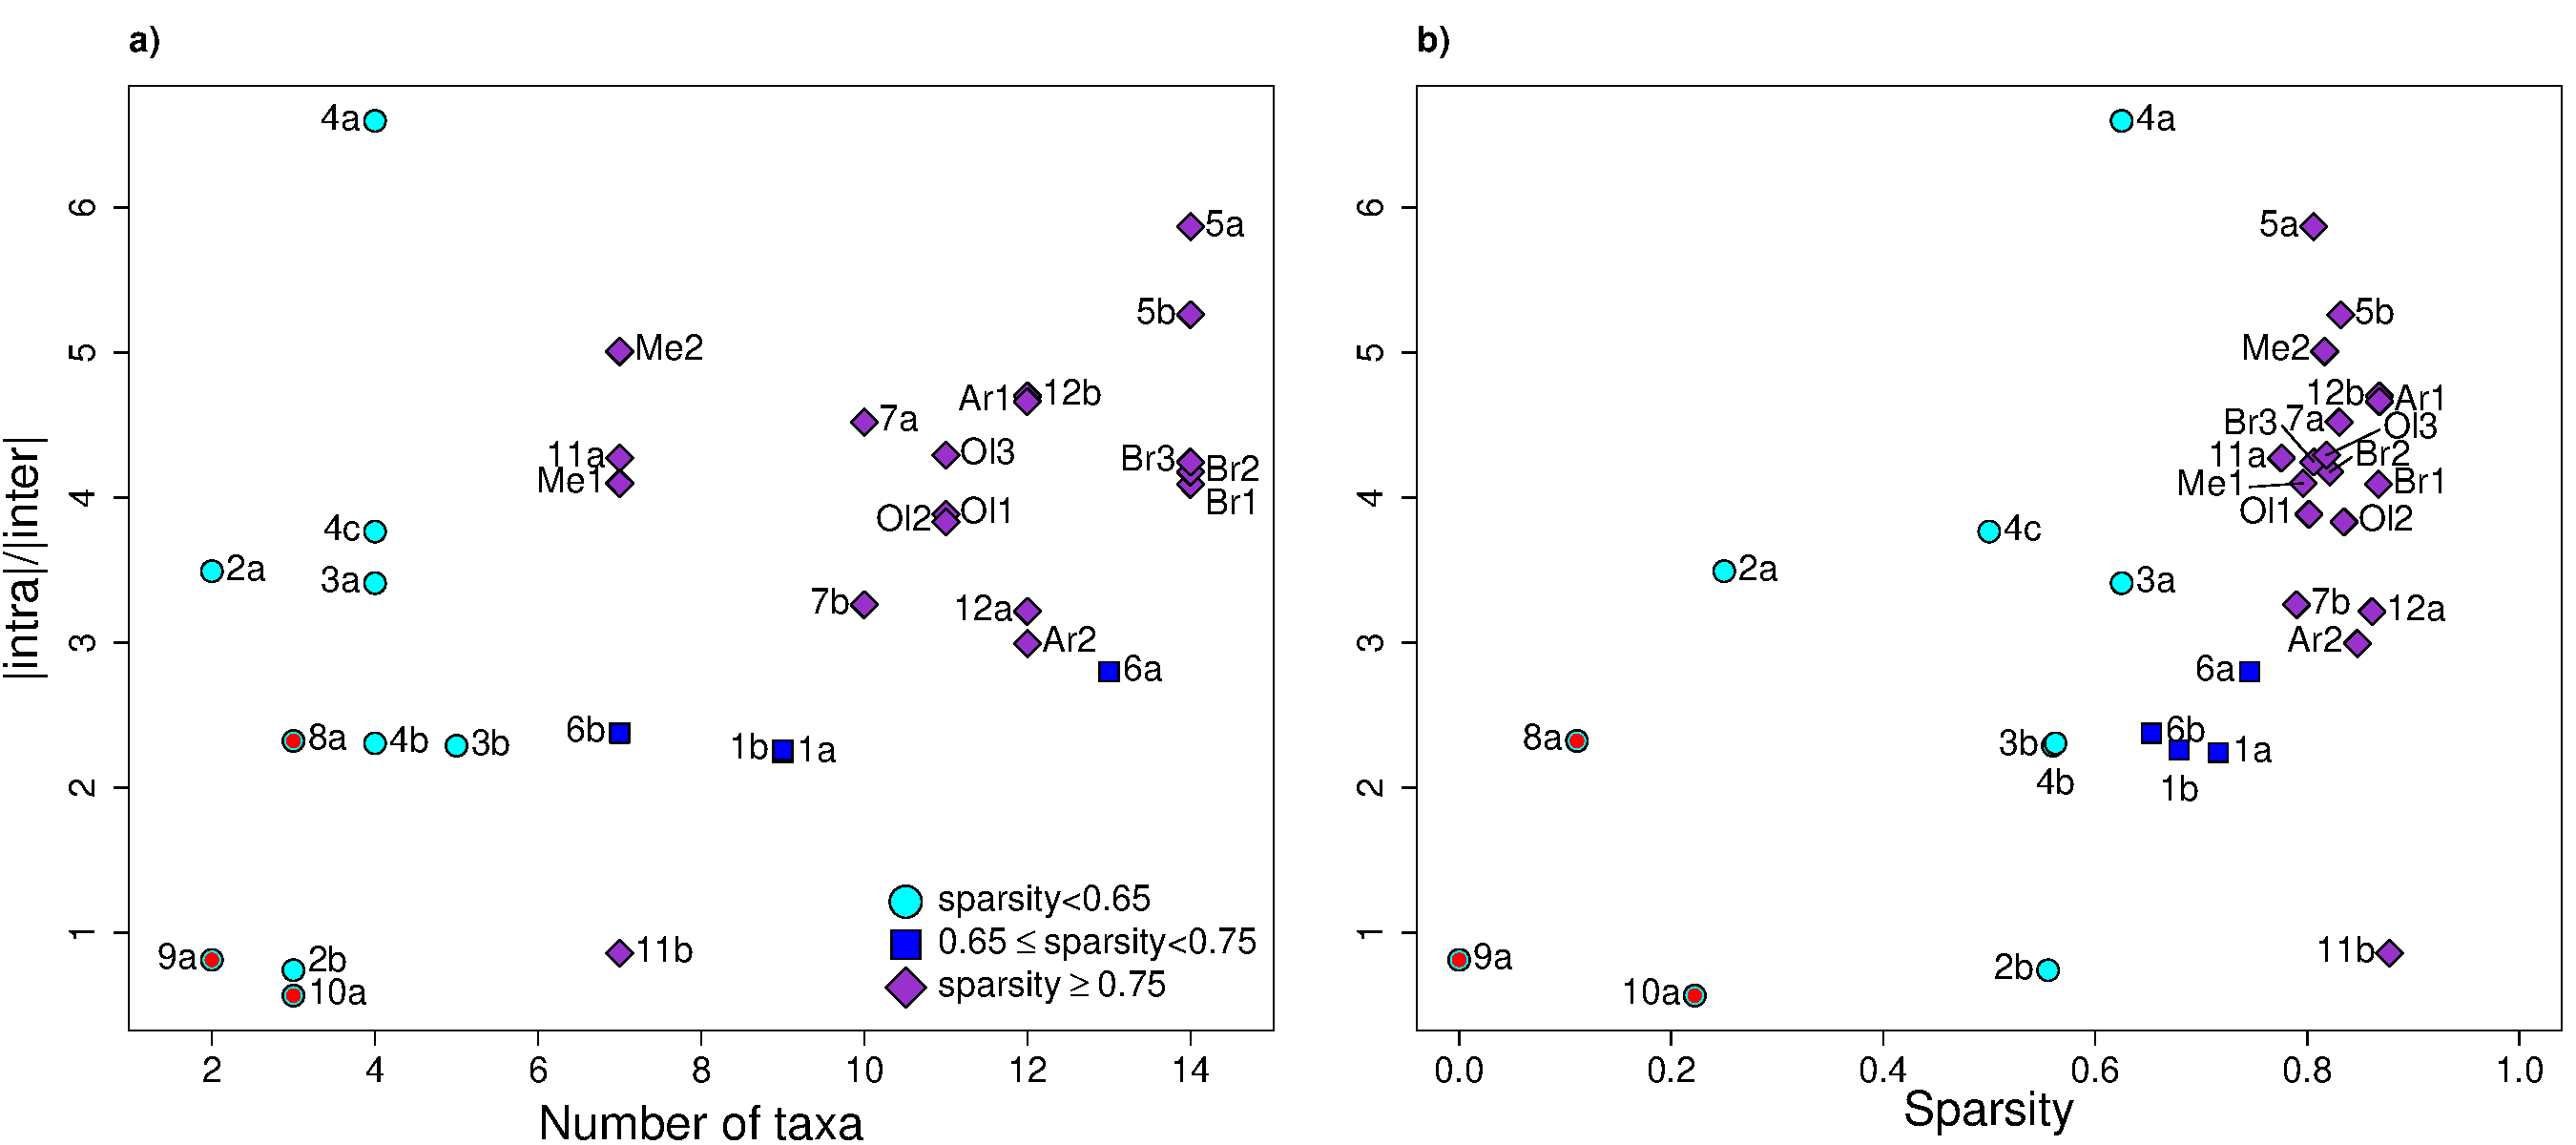
\includegraphics[width=1\textwidth]{comparaison_ratio_code_nolog_cleaner_ONLY_SIGNIF}
\par\end{centering}
\caption{\textbf{Ratio of intra-to-intergroup interaction strength in MAR(1)
studies. }Only significant values are taken into account and missing
values in the matrix are not considered (e.g., not replaced by 0 as
they are in the main text). The color and shape of each point are
a function of the sparsity of the interaction matrix $\mathbf{B}\lyxmathsym{\textendash}\mathbf{I}$
and the relation between the ratio and the sparsity of the matrix
is given in the right panel. Red dots correspond to terrestrial and/or low dimension, predator-prey systems, giving a lower bound for the intra/inter ratio. Corresponding studies are described in
Table \ref{tab:Studies}. \label{fig:Ratio-of-intra-to-intergroup}}
\end{figure}

\begin{figure}[H]
\begin{centering}
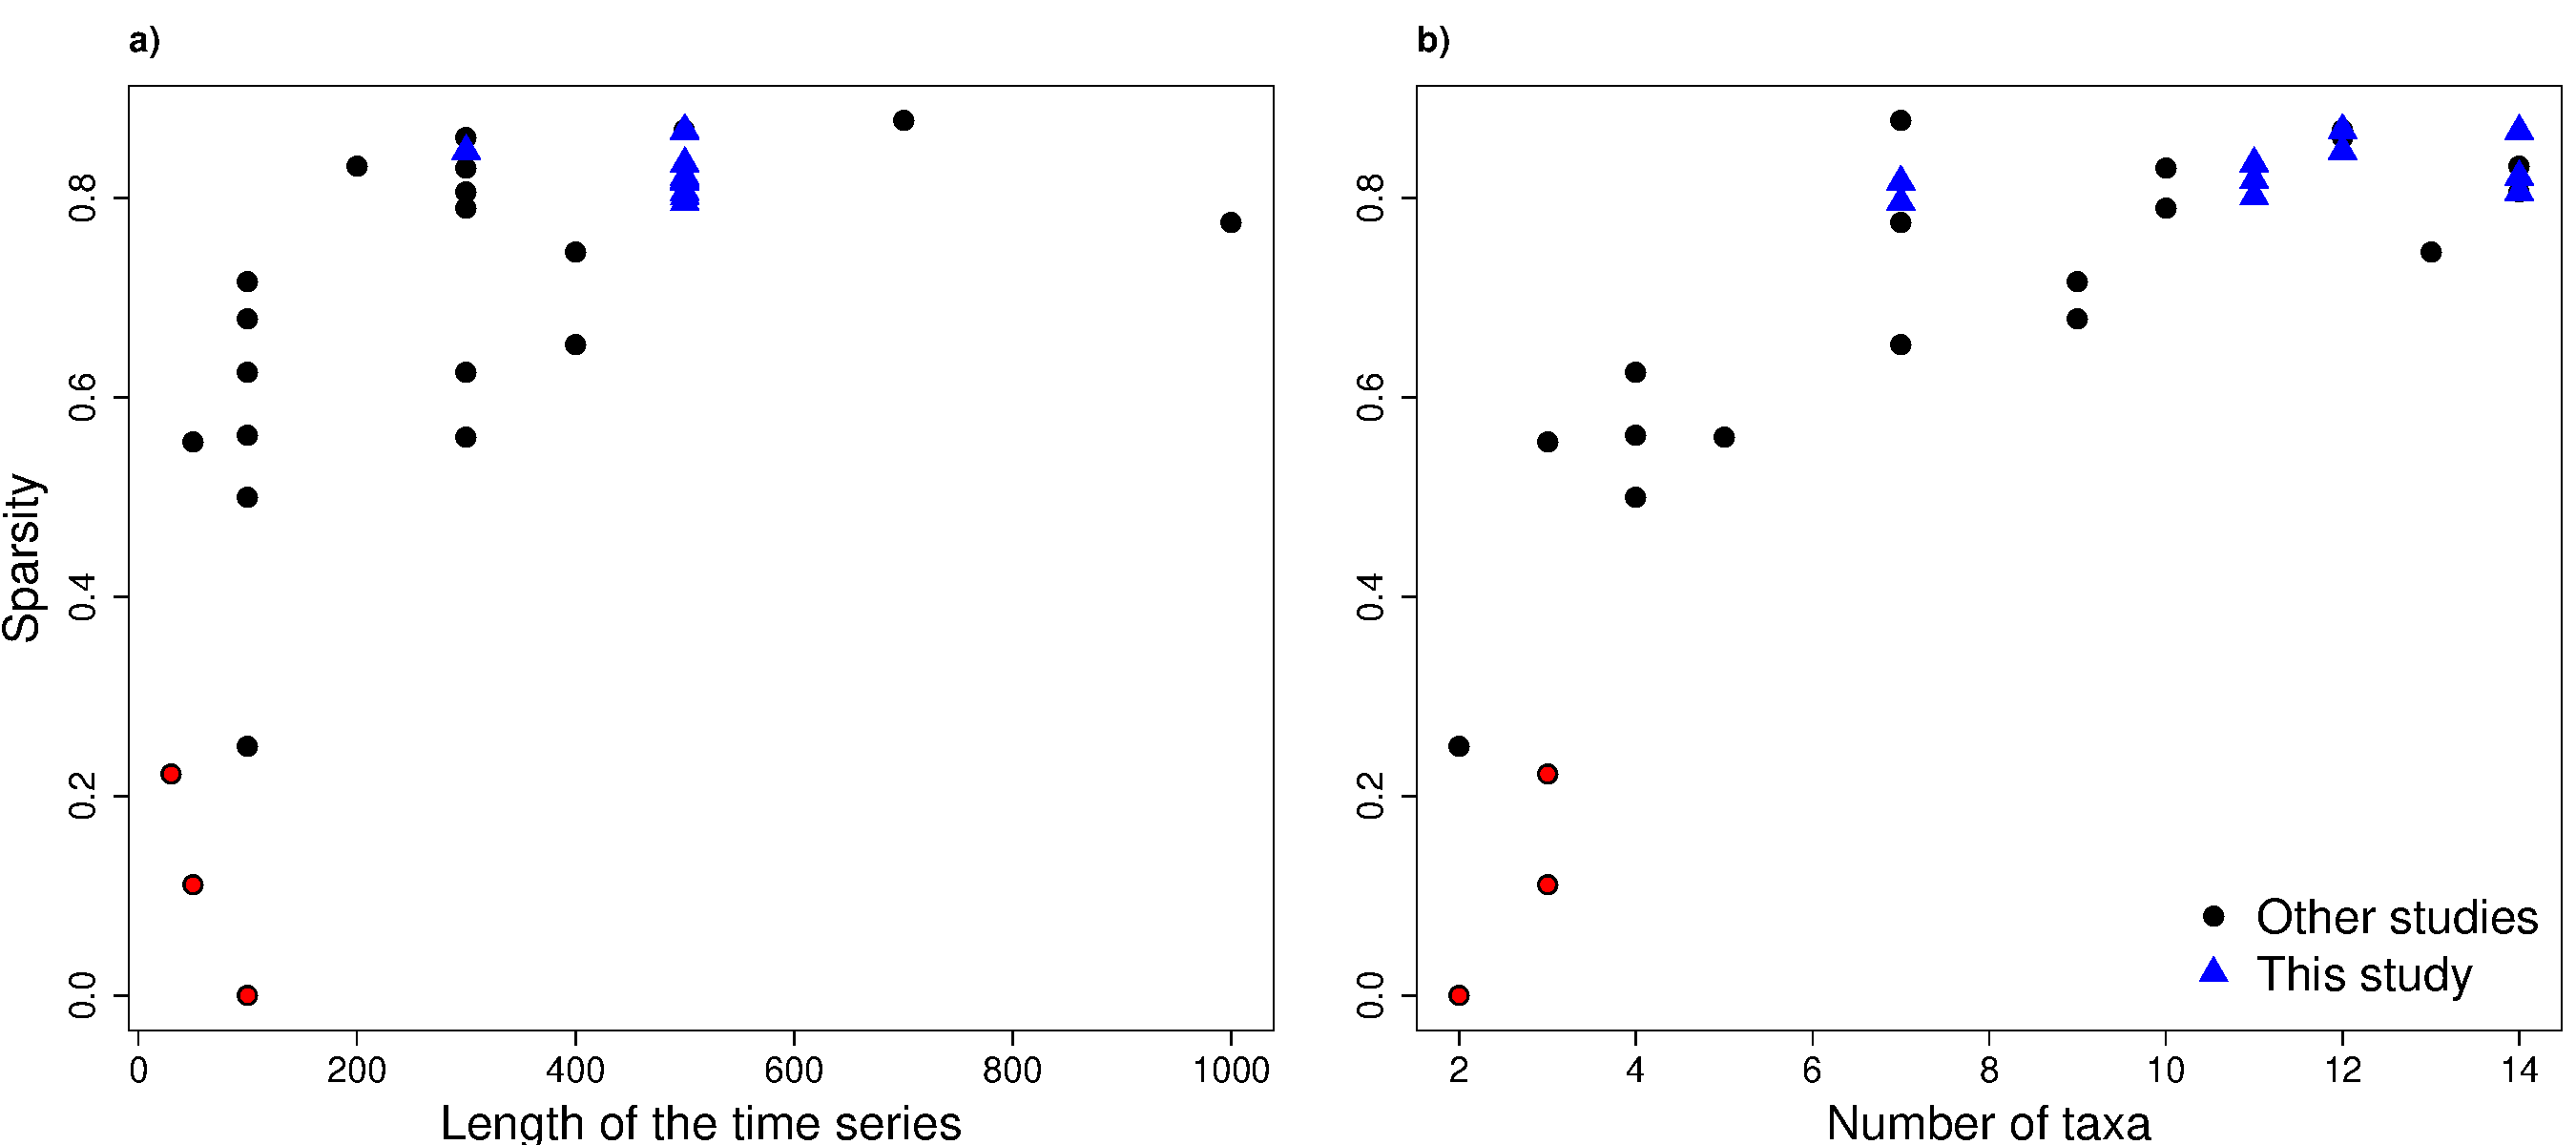
\includegraphics[width=1\textwidth]{sparsity_vs_others_species2taxa}
\par\end{centering}
\caption{\textbf{Relation between interaction sparsity and study design} in
studies described in Table \ref{tab:Studies}. Red dots correspond to terrestrial and/or low dimension, predator-prey systems, giving a lower bound for the intra/inter ratio. Blue triangles correspond
to the present study. \label{fig:ratio_meta}}
\end{figure}

\newpage{}	

\subsection*{Connection to continuous-time models}

{\color{blue} The relation between complexity and stability in community models has been debated in theoretical ecology for decades \citep{may_will_1972, allesina_stabilitycomplexity_2015}. In the field of ecology, random matrix theory has been mostly applied for continuous-time interaction models (\citealt{allesina_stabilitycomplexity_2015}, but see \citealt{cohen_stability_1984}). Here, we intend to connect our statistical discrete-time models to the continuous-time models of stability theory. The discrete log-linear model writes $\mathbf{x}_{t+1} = \mathbf{B} \mathbf{x}_{t}$ in the main text. This model can only approximate continuous-time, possibly non-linear dynamics. There are at least two ways to relate discrete-time models to these dynamics. 

The first approach is to linearize continuous-time dynamics ($\text{d}\mathbf{x}=\mathbf{A}\mathbf{x}\text{dt}$ where $\mathbf{A}$ is the continuous-time community matrix) and integrate the system over time. In this case, the map from one time-step to the other can be written $\mathbf{x}_{t+1} = \text{e}^{\mathbf{A}} \mathbf{x}_{t}$. The discrete-time equivalent of the community matrix $\mathbf{A}$ is then $\mathbf{\log(B)}$ where $\text{e}^{\mathbf{A}}$ is a matrix exponential and $\mathbf{\log(B)}$ the reciprocal of $\text{e}^{\mathbf{A}}$ with $\mathbf{B}$ defined as above. 

The second approach is to first integrate a continuous-time model over a time-step and then linearize the system. In this case, the equivalent matrix $\mathbf{A} = \mathbf{B}-\mathbf{I}$ because it describes the effects of densities on population growth rates (by contrast $\mathbf{B}$ describes effects of log-densities at time $t$ to log-densities at time $t+1$). The second approach is illustrated in more detail in the next section of the Supporting Information. \\

Moreover, the measure of resilience differs in discrete- and continuous-time models. In discrete-time models, and therefore in this study, resilience is measured as the maximum modulus of the eigenvalues of the community matrix ($\max(|\lambda_B|)$), through the dominant eigenvalue of $\mathbf{B}$. In continuous-time models, resilience is linked to the maximum real part of the eigenvalues ($\max(\text{Re}(\lambda_A))$), \textit{i.e.} the real part the leading eigenvalue of $\mathbf{A}$. There is therefore a link to be made between these metrics. We present  Fig.~\ref{fig:comparison_fig} the relationship between resilience metrics $\max(|\lambda_B|)$ and $\max(\text{Re}(\lambda_A))$ to make sure that our results in discrete time consistent with continuous-time theory.

\begin{figure}[H]
    \centering
    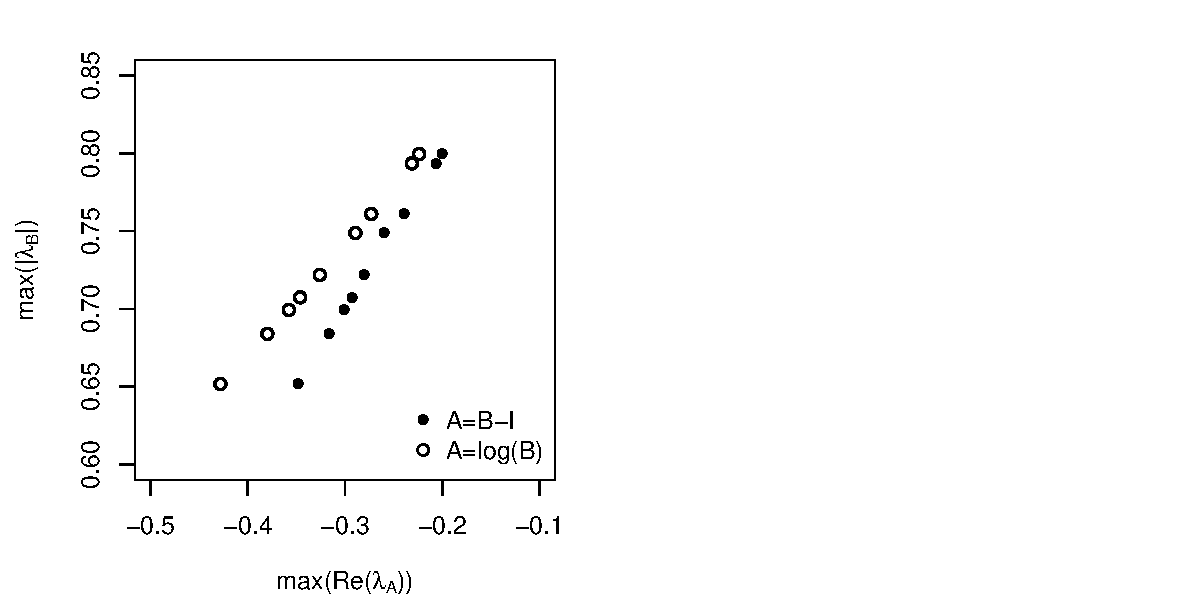
\includegraphics[width=0.99\textwidth]{modB_f_maxReA.pdf}
    \caption{Relationship between discrete-time stability metrics and their continuous-time equivalents (a); relationship between $\max(\text{Re}(\lambda_A))$ and an index of complexity, that is the variance of the off-diagonal coefficients weighted by the number of species in each community in (b).}
    \label{fig:comparison_fig}
\end{figure}

We see in Fig. \ref{fig:comparison_fig} that:
\begin{itemize}
\item leading eigenvalues of $\mathbf{A}$ are similar  for $\mathbf{A} = \mathbf{B}-\mathbf{I}$ and $\mathbf{A} = \mathbf{\log(B)}$ (the difference is around 0.04 for values between -0.45 and -0.2. Hence, $\mathbf{B}-\mathbf{I}$ is a simpler approximation of $\mathbf{A}$ (Fig~\ref{fig:comparison_fig} a)
\item the dominant eigenvalue of $\mathbf{B}$ is strongly correlated to the leading eigenvalue of $\mathbf{A} =\mathbf{B}-\mathbf{I}$ and $\mathbf{A} = \mathbf{\log(B)}$ ($>0.99$ in both cases), which means that our results are compatible with continuous-time theory (Fig~\ref{fig:comparison_fig} a)
\item there is no apparent relationship between stability/resilience for a continuous-time equivalent of $\mathbf{B}$ and complexity (measured as number of species times the variance of the intergroup interaction coefficients) (Fig~\ref{fig:comparison_fig} b).
\end{itemize}

We therefore consider our results on the absence of relation between stability and complexity to be robust to variations in model framework.
}



\subsection*{Connection to Lotka-Volterra competition dynamics}

The Beverton-Holt multispecies competition model, whose variants are
widely used for modelling plant community dynamics \citep{levine_importance_2009,kraft_plant_2015},
is the closest discrete time equivalent to the continuous-time Lotka-Volterra
model (see \citealt{cushing_discrete_2004}; although the mapping is not
perfect for $n\geq3$, \citealt{roeger_discrete_2004}). The Beverton-Holt
multispecies competition model writes

\begin{equation}
N_{i,t+1}=\frac{e^{r_{i}}N_{i,t}}{1+\sum_{j}\alpha_{ij}N_{j,t}}\label{eq:BevHolt}
\end{equation}

where $N_{i,t}$ is the abundance of species $i$ at time $t$, $r_{i}$
is its growth rate and $\alpha_{ij}$ is the effect of species $j$
on species $i$. Here, we show how the interaction strengths $\alpha_{ij}$
map to those of the MAR(1) models used in the main text.

We start with a 2 species model for simplicity, and we note the equilibrium
values of species 1 and 2 as $N_{1}$ and $N_{2}$ (without time subscript).
We re-write the model at equilibrium.

\begin{equation}
\begin{cases}
R_{1}= & \alpha_{11}N_{1}+\alpha_{12}N_{2}\\
R_{2}= & \alpha_{21}N_{1}+\alpha_{22}N_{2}
\end{cases},\textrm{with}\begin{cases}
R_{1}= & e^{r_{1}}-1\\
R_{2}= & e^{r_{2}}-1
\end{cases}
\end{equation}

\begin{equation}
\Leftrightarrow\begin{cases}
\alpha_{21}R_{1}= & \alpha_{21}\alpha_{11}N_{1}+\alpha_{21}\alpha_{12}N_{2}\\
\alpha_{11}R_{2}= & \alpha_{11}\alpha_{21}N_{1}+\alpha_{11}\alpha_{22}N_{2}
\end{cases}
\end{equation}

\begin{equation}
\Leftrightarrow\begin{cases}
N_{1}= & \frac{\alpha_{12}R_{2}-\alpha_{22}R_{1}}{\alpha_{12}\alpha_{21}-\alpha_{22}\alpha_{11}}\\
N_{2}= & \frac{\alpha_{21}R_{1}-\alpha_{11}R_{2}}{\alpha_{12}\alpha_{21}-\alpha_{22}\alpha_{11}}
\end{cases}\label{eq:N1N2}
\end{equation}

Setting $n=\log(N)$, eq. \ref{eq:BevHolt} is equivalent to

\begin{equation}
\begin{cases}
n_{1,t+1}= & r_{1}+n_{1,t}-\ln(1+\alpha_{11}N_{1,t}+\alpha_{12}N_{2,t})\\
n_{2,t+1}= & r_{2}+n_{2,t}-\ln(1+\alpha_{21}N_{1,t}+\alpha_{22}N_{2,t})
\end{cases}
\end{equation}

We want to compute $J$, the log-scale Jacobian matrix of the model.
Let us note $X=\ln(1+\alpha_{11}N_{1}+\alpha_{12}N_{2})$ and $Y=\ln(1+\alpha_{12}N_{1}+\alpha_{22}N_{2})$.

\begin{equation}
J=\left(\begin{array}{cc}
1-\frac{\partial X}{\partial n_{1}} & -\frac{\partial X}{\partial n_{2}}\\
-\frac{\partial Y}{\partial n_{1}} & 1-\frac{\partial Y}{\partial n_{2}}
\end{array}\right)
\end{equation}

We have $\frac{\partial X}{\partial n_{1}}=\frac{\partial X}{\partial N_{1}}\frac{\partial N_{1}}{\partial n_{1}}=\frac{\alpha_{11}}{1+\alpha_{11}N_{1}+\alpha_{12}N_{2}}e^{n_{1}}=\frac{\alpha_{11}}{1+\alpha_{11}N_{1}+\alpha_{12}N_{2}}N_{1}$,
which leads to

\begin{equation}
J-I=\left(\begin{array}{cc}
-\frac{\alpha_{11}N_{1}}{1+\alpha_{11}N_{1}+\alpha_{12}N_{2}} & -\frac{\alpha_{12}N_{2}}{1+\alpha_{11}N_{1}+\alpha_{12}N_{2}}\\
-\frac{\alpha_{21}N_{1}}{1+\alpha_{21}N_{1}+\alpha_{22}N_{2}} & -\frac{\alpha_{22}N_{2}}{1+\alpha_{21}N_{1}+\alpha_{22}N_{2}}
\end{array}\right)
\end{equation}

For this demonstration, we consider diffuse competition, that is

\begin{equation}
\begin{cases}
\alpha_{ii}= & k\alpha\\
\alpha_{ij}= & \alpha,\forall i\neq j
\end{cases}\label{eq:diffuse_comp}
\end{equation}

If we combine eq. \ref{eq:N1N2} and eq. \ref{eq:diffuse_comp}, we
have

\begin{equation}
\begin{cases}
N_{1}= & \frac{\alpha R_{2}-k\alpha R_{1}}{\alpha^{2}-k^{2}\alpha^{2}}\\
N_{2}= & \frac{\alpha R_{1}-k\alpha R_{2}}{\alpha^{2}-k^{2}\alpha^{2}}
\end{cases}
\end{equation}

and
\begin{equation}
J-I=\left(\begin{array}{cc}
-\frac{k\alpha N_{1}}{1+k\alpha N_{1}+\alpha N_{2}} & -\frac{\alpha N_{2}}{1+k\alpha N_{1}+\alpha N_{2}}\\
-\frac{\alpha N_{1}}{1+\alpha N_{1}+k\alpha N_{2}} & -\frac{k\alpha N_{2}}{1+\alpha N_{1}+k\alpha N_{2}}
\end{array}\right)
\end{equation}

\begin{equation}
\Rightarrow\begin{cases}
(J-I)_{11}= & \frac{-\frac{k}{1-k^{2}}(R_{2}-kR_{1})}{1+\frac{k}{1-k^{2}}(R_{2}-kR_{1})+\frac{1}{1-k^{2}}(R_{1}-kR_{2})}\\
(J-I)_{12}= & \frac{-\frac{1}{1-k^{2}}(R_{1}-kR_{2})}{1+\frac{k}{1-k^{2}}(R_{2}-kR_{1})+\frac{1}{1-k^{2}}(R_{1}-kR_{2})}
\end{cases}\Rightarrow(J-I)_{11}=k\frac{R_{2}-kR_{1}}{R_{1}-kR_{2}}(J-I)_{12}
\end{equation}

By symmetry, we can also write

\begin{equation}
(J-I)_{22}=k\frac{R_{1}-kR_{2}}{R_{2}-kR_{1}}(J-I)_{21}
\end{equation}

The same reasoning can actually be applied
with $n$ species as the Jacobian has a similar form.

\begin{equation}
\begin{aligned}(J-I)_{ii} & = & \frac{-\alpha_{ii}N_{i}}{1+\sum_{j}\alpha_{ij}N_{j}}\\
 & = & \frac{-k\alpha N_{i}}{1+k\alpha N_{i}+\sum_{j,j\neq i}\alpha N_{j}}
\end{aligned}
\end{equation}

and

\begin{equation}
\begin{aligned}(J-I)_{ij} & = & \frac{-\alpha_{ij}N_{j}}{1+\sum_{l}\alpha_{il}N_{l}}\\
 & = & \frac{-\alpha N_{j}}{1+k\alpha N_{i}+\sum_{l,l\neq i}\alpha N_{l}}\\
 & = & (J-I)_{ii}\frac{\alpha N_{j}}{k\alpha N_{i}}\\
 & = & \frac{1}{k}(J-I)_{ii}\frac{N_{j}}{N_{i}}
\end{aligned}
\end{equation}

Therefore, unless the growth rates and the resulting abundances differ
over several orders of magnitude, the strength of the competition
ratio $k$ should be roughly comparable between MAR(1) and Lotka-Volterra
or Beverton-Holt models. {\color{blue}  Unfortunately, in this paper, the mean and median ratio between pairs of abundances are respectively 6 and 23, with values between 1.01 and 439.5. Thus, the order of magnitude between interaction strengths might change, depending on the species in presence. The mapping between Lotka-Volterra and MAR interaction strength ratios is therefore non-trivial, especially in highly uneven communities.}

\bibliography{phytoInteractions_ref,bib_fig_review}

\end{document}
